% ***************************** MAIN FILE **********************************

\documentclass[12pt]{report}           % Art des zu erstellenden Dokuments
% bei zweiseitigem Druck twoside-Option oder book-Klasse verwenden

% ****************************** PREAMBLE **********************************
% **************************** PACKAGE SETUP *******************************
\usepackage[ngerman]{babel}          % Lokalisierung von Typographie, Silbentrennung, etc.
\usepackage{geometry}                % Zum Gestallten der Seiten
\usepackage{ucs}                     % Erweiterte Unterstützung von UTF-8-Kodierung
\usepackage[utf8x]{inputenc}         % Unterstützung von UTF-8 in Eingabe-Dateien
\usepackage[T1]{fontenc}             % Zeichensatzkodierung von LaTeX (Cork-Kodierung)
\usepackage{helvet,courier,mathptmx} % Verwendete Schriftarten

\usepackage{amsmath}                 % Mathematische Infrastruktur für LaTeX der AMS
\usepackage{amsfonts}                % Mathematische Schriftarten
\usepackage{amssymb}                 % Mathematische Symbole
\usepackage{amsthm}                  % Erweiterung der Theorem-Umgebungen

\usepackage{fancyhdr}                % Erweiterte Konfiguration von Kopf/Fußzeile
\usepackage{hyperref}                % Querverweise, Hyperlink, pdf-Konfiguration, etc.
\usepackage[
nonumberlist, %keine Seitenzahlen anzeigen
nopostdot,    %Den Punkt am Ende jeder Beschreibung deaktivieren
acronym,      %ein Abkürzungsverzeichnis erstellen
toc,          %Einträge im Inhaltsverzeichnis
section,      %im Inhaltsverzeichnis auf section-Ebene erscheinen
%numberedsection=autolabel %Zum einfügen in das Appendix
]{glossaries}					     % vor hyperref einbinden, um Verlinkung zu deaktiveren

\usepackage{float}                   % Selbstdefinierte Floating-Umbgebungen
\usepackage{tabularx}                % Tabellen mit einstellbarer Spaltenbreite
\usepackage[labelfont=bf]{caption}   % Anpassen der Abbildungs- und Tabellenbeschriftungen

\usepackage{algpseudocode}           % Algorithmen als Pseudocode (basiert auf algorithmicx)
\usepackage{listings}                % Quellcode-Satz (z.B. mit Syntax-Hervorhebung)

\usepackage{graphicx}                % Erweiterte Unterstützung von Graphiken
\usepackage{textpos}                 % Beliebig platzierte Textboxen
\usepackage{xcolor}                  % TeX-Engine-unabhängige Definition von Farben

\usepackage[numbers]{natbib}         % Weiter Optionen für die Bibliographie

\usepackage{setspace}
\usepackage{ellipsis}	% Korrigiert den Wei�raum um Auslassungspunkte
\usepackage{placeins} 
\usepackage{tikz}

% ****************************** TOP MATTER ***********************************
\renewcommand{\author}{Stefan Kruk}           % Name
\newcommand{\dateOfBirth}{14.08.1992}           % Geburtsdatum
\newcommand{\matrNumber}{7084972}              % Matrikelnummer
\newcommand{\studycourse}{Softwaretechnik (Dual)}           % Studiengang

\newcommand{\supervisor}{Prof. Dr. Johannes Ecke-Schüth} % Betreuer
\newcommand{\institution}{Fachhochschule Dortmund} % Hochschule
\newcommand{\faculty}{Informatik}               % Fachbereich
\newcommand{\toponym}{Dortmund}                 % Ort

\newcommand{\subject}{Projektarbeit}  % Art/Thema der Arbeit
\newcommand{\titel}{Gemeinsamkeiten und Unterschiede von Software-Orientierte-Architektur (SOA) und Microservices} % Titel der Arbeit
%\newcommand{\subtitel}{Zweizeiliger Untertitel\\sofern vorhanden} % Untertitel
\newcommand{\degree}{Bachelor/Master of Art\xspace} % Angestrebter Titel (nur bei Abschlussarbeiten, sonst leer lassen/auskommentieren)

\newcommand{\keywords}{Projektarbeit, SOA, Microservices, Informatik, {FH Dortmund}} % Stichworte (durch Komma getrennt)

% **************************** HYPERREF SETUP *******************************
\definecolor{linkcolor}{rgb}{1,0.5,0}
\hypersetup
{
bookmarks=true,                        % Lesezeichen im PDF erzeugen
bookmarksopen=true,                    % Lesezeichen im PDF sofort anzeigen
backref=true,                          % Rückverweise im Literaturverzeichnis
colorlinks=true,                       % Farbige Verweise
%hidelinks = true,                      % Verweise verbergen (entfernt Farbe und Rahmen)
pdfstartview={FitH},                   % Ansicht des PDFs beim öffnen
pdftitle={\titel},                     % Title des PDFs
pdfauthor={\author , \supervisor},     % Autor des PDFs
pdfsubject={\subject},                 % Thema des PDFs
%pdfcreator={Creator},                 % Erzeuger des Dokuments (Anwendungsprogramm)
%pdfproducer={Producer},               % Ersteller des PDFs (Programm/Bibliothek/Skript)
pdfkeywords={\keywords},               % Stichwörter zum PDF
linkcolor=linkcolor,                   % Farbe von Querverweisen
citecolor=orange,                       % Farbe von Zitaten
filecolor=magenta,                     % Farbe von Verweisen auf Dateien
urlcolor=cyan                          % Farbe von URLs
}
% Weitere Optionen: http://www.tug.org/applications/hyperref/manual.html

% Für Zeichnungen
\usetikzlibrary{% 
    arrows,% 
    calc,% 
    fit,% 
    patterns,% 
    plotmarks,% 
    shapes.geometric,% 
    shapes.misc,% 
    shapes.symbols,% 
    shapes.arrows,% 
    shapes.callouts,% 
    shapes.multipart,% 
    shapes.gates.logic.US,% 
    shapes.gates.logic.IEC,% 
    er,% 
    automata,% 
    backgrounds,% 
    chains,% 
    topaths,% 
    trees,% 
    petri,% 
    mindmap,% 
    matrix,% 
    calendar,% 
    folding,% 
    fadings,% 
    through,% 
    positioning,% 
    scopes,% 
    decorations.fractals,% 
    decorations.shapes,% 
    decorations.text,% 
    decorations.pathmorphing,% 
    decorations.pathreplacing,% 
    decorations.footprints,% 
    decorations.markings,% 
    shadows
} 

% **************************** LISTINGS SETUP *******************************
\definecolor{keywords}{rgb}{0.5 0 0.3}
\definecolor{comments}{rgb}{0.25,0.5,0.37}
\definecolor{lila}{RGB}{112, 6, 147}
\definecolor{kommentgreen}{RGB}{5,132,71}
\definecolor{grey}{RGB}{242,242,242}  
\definecolor{darkgreen}{named}{green}
\definecolor{darkblue}{named}{blue}
\definecolor{lightblue}{RGB} {63,95,191}
\definecolor{darkred}{named}{red}
\definecolor{grau}{named}{gray}
\definecolor{fh_orange}{rgb}{0.953,0.201,0}
\definecolor{fh_grau}{rgb}{0.76,0.75,0.76}

\definecolor{listinggray}{gray}{0.9}
\definecolor{lbcolor}{rgb}{0.9,0.9,0.9}
\lstset{literate=%
    {Ö}{{\"O}}1
    {Ä}{{\"A}}1
    {Ü}{{\"U}}1
    {ß}{{\ss}}1
    {ü}{{\"u}}1
    {ä}{{\"a}}1
    {ö}{{\"o}}1
    {~}{{\textasciitilde}}1
}
\lstset{ %
    backgroundcolor=\color{grey},   % Hintergrundfarbe
    basicstyle=\linespread{0.94}\footnotesize\ttfamily, % Schrifteinstellungen für Quellcode
    breakatwhitespace=false,         % Automatische Zeilenumbrüche nur bei Leer- oder Tabulatorzeichen (Leerraum/whitespaces)
    breaklines=true,                 % Automatische Zeilenumbrüche
    captionpos=b,                    % Beschriftung unten
    commentstyle=\color{comments},   % Schrifteinstellungen für Kommentare
    columns=felxible,                 % Ist notwendig, damit man Quellcode aus den Listings kopieren kann
    %  deletekeywords={...},            % Bestimmte Schlüsselwörter entfernen
    escapeinside={\%*}{*)},          % Defintion von Escape-Sequenzen
    extendedchars=false,                   % Nicht ASCII-Zeichen erlauben
    frame=single,                    % Rahmen um den Quellcode
    keepspaces=true,                 % Einrückungen im Quellcode behalten
    keywordstyle=\bfseries\color{keywords},% Schrifteinstellungen für Schlüsselwörter
    language=java,                   % Programmiersprache des Quellcodes
    %  morekeywords={*,...},            % Zusätzliche Schlüsselwörter
    numbers=left,                    % Zeilennummerierung
    numbersep=5pt,                   % Abstand zwischen Zeilennummerierung und Quellcode
    numberstyle=\color{black}, % Schrifteinstellungen für Zeilennummern
    rulecolor=\color{black},         % if not set, the frame-color may be changed on line-breaks within not-black text (e.g. comments (green here))
    showspaces=false,                % Leerraum-Zeichen anzeigen
    showstringspaces=false,          % Leerzeichen in Zeichenketten anzeigen
    showtabs=false,                  % Tabulatorzeichen in Zeichenketten anzeigen
    stepnumber=1,                    % Schrittweite bei Zeilennummern
    stringstyle=\color{blue},        % Schrifteinstellungen für Zeichenketten
    tabsize=4,                       % Tabulatorbreite (Anzahl Leerzeichen)
    numberbychapter=false            % Nummeriere Quellcode fortlaufend je Kapitel
}

\lstdefinestyle{java}
{
    language=Java,
    keywordstyle=\bfseries\color{lila},  	% underlined bold black keywords 
    identifierstyle=\bfseries\color{blue}, 
    commentstyle=\bfseries\color{kommentgreen}, % white comments 
    stringstyle=\bfseries\color{black},
}

\lstdefinestyle{xml}
{
    language=xml,
    basicstyle=\fontsize{9pt}{9pt}\selectfont\color{kommentgreen},
    keywordstyle=\color{lila},  	% underlined bold black keywords 
    %Hier können bei Bedarf noch weitere Keywords eingetragen werden
    keywords={name, value, version, encoding, id, type, xmlns:xsi, ref, namespace},
    identifierstyle=\color{black},  
    stringstyle=\color{blue},  
    commentstyle=\color{lightblue},
    morecomment=[s]{<!--}{-->},
    rulecolor=\color{black}
}
\renewcommand{\lstlistlistingname}{Quellcode}
\renewcommand{\lstlistingname}{Quellcode}

\AtBeginDocument{\numberwithin{lstlisting}{section}} % Nummeriere Quellcode fortlaufend je Abschnitt

% ************************** HEADER/FOOTER SETUP ****************************
\setlength{\headheight}{15pt}

\renewcommand{\chaptermark}[1]{ \markboth{#1}{} }

\fancyhf{}
\fancyhead[LE]{\thepage \ \ \ \ {\tiny \author, \today}}
\fancyhead[RO]{{\tiny \author, \today} \ \ \ \ \thepage}
\fancyhead[LO,RE]{\textit{\nouppercase{\leftmark}} }
\renewcommand{\headrulewidth}{0pt}

% **************************** GRAPHICX SETUP *********************************
\DeclareGraphicsExtensions{.pdf,.png,.jpg} % bekannte Graphik-Dateiformate (müssen nicht mehr im Dateinamen angegeben werden, also statt "beispiel.png" nur noch "beispiel")
\graphicspath{{./figure/}}   % path to graphics folder, usage {PATH},{ANOTHERPATH}...

% ************************** BIBLIOGRAPHY SETUP ********************************
\bibliographystyle{dinat}    % Literaturverzeichnis nach DIN
%\AtBeginDocument{\nocite{*}}    % Diese Zeile vor der Abgabe der Arbeit entfernen!

% ****************************** MATH SETUP ************************************
\everymath{\displaystyle}    % Erzwinge \displaystyle für Mathematischen-Modus


% ************************* THEOREMS AND PROOF *********************************
\newtheoremstyle{thesis}     % Name des neuen Theorem-Stils
{3pt}                        % Abstand oberhalb des Theorems
{3pt}                        % Abstand unterhalb des Theorems
{\itshape}                   % Schrifteinstellungen innerhalb des Theorems
{}                           % Einrückung der Theorem-Überschrift
{\bfseries}                  % Schrifteinstellungen für die Überschrift des Theorems
{}                           % Satzzeichen zwischen Überschrift und Theorem-Rumpf
{\newline}                   % Abstand hinter der Überschrift
{}                           % Spezifikation der Überschrift
  
\theoremstyle{thesis}        % Verwende neuen Theorem-Stil

\newtheorem{theorem}{Satz}[section] % neue Theorem-Umgebung: theorem (Satz)
\providecommand*{\theoremautorefname}{Satz} % autoref-Name für theorem

\newtheorem{definition}{Definition}[section] % neue Theorem-Umgebung: definition (Definition)
\providecommand*{\definitionautorefname}{Definition} % autoref-Name für definition

\renewcommand{\qedsymbol}{$\blacksquare$} % Schwarzes Quardrat als Symbol für: q. e. d.
\renewenvironment{proof}[1][\proofname]{{\bfseries #1:}~}{\qed} % "Beweise:" in Fettdruck

% *************************** PSEUDOCODE SETUP ********************************
\floatstyle{boxed}                        % Rahmen für pseudocode-Umgebung
\newfloat{pseudocode}{htbp}{lop}[section] % Definieren pseudocode-Umgebung
\floatname{pseudocode}{Pseudocode}        % Beschrifte pseudocode-Umgebung mit "Pseudocode"

\newcommand{\listofpseudocodename}{Pseudocodeverzeichnis}
\newcommand{\listofpseudocode}{\listof{pseudocode}{\listofpseudocodename}}
\providecommand*{\pseudocodeautorefname}{Pseudocode}

% ******************************* PAGE SETUP **********************************
\textheight23cm
\textwidth14cm
\voffset0cm
\topskip0cm
\topmargin-1.2cm
\headheight1.0cm
\headsep1.5cm
\oddsidemargin1.0cm
\evensidemargin1.0cm
\renewcommand{\baselinestretch}{1.4} 
\widowpenalty=300
\clubpenalty=300

% ******************************** MACROS *************************************
\newcommand{\RR}{\mathbf{R}}
\newcommand{\NN}{\mathbf{N}}
\newcommand{\QQ}{\mathbf{Q}}
\newcommand{\ZZ}{\mathbf{Z}}
\newcommand{\CC}{\mathbf{C}}
\newcommand{\SOA}{Service-orientierte Architektur}
\newcommand{\ebay}{eBay}
\newcommand{\secref}[1]{\ref{#1} \nameref{#1}}

%%%%%%%%%%%%%%%%%%%%%%%%%%%%%%%%%%%%%%%%%%%%%%%%%%%%%%%%%%%%%%%%%%%%%%%%%%%%%%%
% ****************************** Glossarie ************************************
%%%%%%%%%%%%%%%%%%%%%%%%%%%%%%%%%%%%%%%%%%%%%%%%%%%%%%%%%%%%%%%%%%%%%%%%%%%%%%%

%Befehle für Glossar
\newglossaryentry{glos:SOA}{
    name=SOA,
    description={SOA steht für Service-orientierte Architektur und ist ein Architekturmuster für Service-orientierte Systeme. SOA ist in dem Bereich der verteilten Systeme einzuordnen und wird eingesetzt, um Dienste von IT-Systemen zu strukturieren und zu nutzen.}
}

\newglossaryentry{glos:Microservice}{
    name=Microservice, 
    description={Microservices sind ein Architekturmuster aus dem Bereich der verteilten Anwendungen, bei dem komplexe Anwendungen in eigenständige Prozessen zerlegt werden. Diese kommunizieren mit Hilfe von sprachunabhängigen Schnittstellen untereinander. Die Prozesse, welche ebenfalls Microservices genannt werden, sind kleine unabhängige Dienste, welche möglichst nur eine Aufgabe erledigen sollen, diese aber dafür besonders gut. Dadurch ist ein modularer Aufbau von Anwendungssoftware möglich.}
}

\newglossaryentry{glos:Services}{
	name=Services,
	description={Services, zu deutsch Dienste, sind IT-Repräsentanten von fachlichen Funktionalitäten. Dabei sollen Services in sich abgeschlossen (autark) sein, damit diese eigenständig genutzt werden können. Damit Services über das Netzwerk genutzt werden können, müssen wohldefinierte Schnittstellen vorhanden sein. Zusätzlich sollte die Granularität von Services grob sein, um die Abhängigkeiten zu anderen Diensten gering zu halten.}
}

%%%%%%%%%%%%%%%%%%%%%%%%%%%%%%%%%%%%%%%%%%%%%%%%%%%%%%%%%%%%%%%%%%%%%%%%%%%%%%%
% ************************** BEGINN OF DOCUMENT *******************************
%%%%%%%%%%%%%%%%%%%%%%%%%%%%%%%%%%%%%%%%%%%%%%%%%%%%%%%%%%%%%%%%%%%%%%%%%%%%%%%
\begin{document}

\begin{titlepage}
%FH LOGO
% 
\includegraphics[width=3.8cm]{content/images/fh_logo_neu_orange_A4}

% *** Subject ***
{\centering {\Huge \bfseries \subject\par}}
% *** Thema ***
\bigskip\bigskip
{\centering Thema:\\[0.3cm] {\textbf {\large\titel} \\[0.3cm] \ifdefined\subtitel \subtitel  \fi \\[0.05cm]}\par}

\bigskip\bigskip
% *** Author Informationen ***
{\centering\bfseries \author\par}
{\centering geboren am \dateOfBirth\par}
{\centering Matr.-Nr.: \matrNumber\par}


\bigskip\bigskip\bigskip
%*** Hochschulinformationen ***
{\centering An der \institution im Fachbereich \faculty erstellte \par}
{\centering \subject\par}
{\centering im Studiengang \studycourse \par}
 \ifdefined\degree
\bigskip
{\centering   
    zur Erlangung des Grades akademischen Grades \degree \par}
\fi
%*** Betreuer Informationen ***
\bigskip\bigskip\bigskip
{\centering \textbf{Betreuer:} \supervisor \par}

%*** Hochschul Logo
\bigskip\bigskip\bigskip
{\centering  
\includegraphics[width=3.8cm]{content/images/fh_logo_neu_orange_A4} \par}
{\centering\bfseries  Fachbereich \faculty\par}

\bigskip\bigskip
{\centering Dortmund, \today\par}

\end{titlepage}


% ***************************** FRONT MATTER **********************************
\setcounter{page}{1}
\pagenumbering{roman}

\chapter*{Überblick}
\section*{Kurzfassung}
In dieser Arbeit werden die Vor- und Nachteile von \SOA\ und Microservices erörtert und anschließend miteinander verglichen werden. Dabei wird explizit auf die Unterschiede und Gemeinsamkeiten der beiden Architekturmodelle eingegangen werden. Für eine bessere Verständlichkeit wird zusätzlich ein bestimmter Prozesskontext mit beiden Modellen implementiert.

\section*{Abstract}
In this Projekt will be the Pro and Cons of service-oriented architecture and Microservices described. After that both architectural models will be compared. In this Process the differences and similarities between these two models will be described. For a better understanding i will implement an application with both architectural models.

% *************************** TABLE OF CONTENTS *******************************
% ************************* (Inhaltsverzeichnis) ******************************
% Die Auskommentierte Zeile fügt das Inhaltsverzeichnis zum Inhaltsverzeichnis hinzu. Diese Verhalten kann auch über das Paket tocbibind erreicht werden. Allerdings funktioniert das Paket nicht für das Pseudocodeverzeichnis, aus diesem Grund werden die Einträge "manuell" hinzugefügt.

%\phantomsection\addcontentsline{toc}{chapter}{\numberline{}\contentsname}
{
\baselineskip=15pt % Schriftlinien-Abstand 15 pt (nur beim Inhaltsverzeichnis)
\tableofcontents   % Inhaltsverzeichnis einfügen
}
{
\baselineskip=22pt % Schriftlinien-Abstand 22 pt (bei allen anderen Verzeichnissen)

% **************************** LIST OF FIGURES ********************************
% ************************ (Abbildungsverzeichnis) ****************************
%\clearpage\phantomsection\addcontentsline{toc}{chapter}{\numberline{}\listfigurename}

\listoffigures % Abbildungsverzeichnis einfügen

% **************************** LIST OF TABLES *********************************
%\clearpage\phantomsection\addcontentsline{toc}{chapter}{\numberline{}\listtablename}

%\listoftables % Tabellenverzeichnis einfügen

% ************************** LIST OF PSEUDOCODE *******************************
%\clearpage\phantomsection\addcontentsline{toc}{chapter}{\numberline{}\listofpseudocodename}

%\listofpseudocode % Pseudocodeverzeichnis einfügen

% *************************** LIST OF LISTINGS ********************************
%\clearpage\phantomsection\addcontentsline{toc}{chapter}{\numberline{}\lstlistlistingname}

%\lstlistoflistings % Quellcodeverzeichnis einfügen
}

% ******************************* Glossar ************************************
%Alle Glossare ausgeben
%\printglossaries

%Glossar ausgeben
\printglossary[style=altlist,title=Glossar]


%Abkürzungen ausgeben
\deftranslation[to=German]{Acronyms}{Abkürzungsverzeichnis}
\printglossary[type=\acronymtype,style=long]

%Symbole ausgeben
\printglossary[type=symbolslist,style=long]
\newpage

% ***************************** MAIN MATTER ***********************************
\pagestyle{fancy}
\pagenumbering{arabic}

\chapter{Einleitung}
\label{chap:Einleitung}
Die Idee der Aufteilung eines komplexen Softwaresystemes ist nicht neu. Monolithische Systeme bestehen meistens aus mehreren Modulen, welche zusammen zu einer ausführbaren Datei gepackt werden. Es kann jedoch auch möglich, dass Module in eigene Bibliotheken verpackt werden, welche zur Laufzeit geladen werden. Da die Bibliotheken für die korrekte Ausführung der Software notwendig sind, müssen diese mit ausgeliefert werden. Müssen einzelne Programmteile verändert (korrigiert, erweitert, angepasst oder verbessert) werden, muss jede Software, welche diesen Programmteil verwendet neu gebaut und ausgeliefert werden. Dies kann einen erheblichen Aufwand bedeuten, wenn dieser Programmteil in einer großen Anzahl von Software verwendet wird. Daher wurde die Idee entwickelt, Fachlichkeiten in einzelne Dienste (Services) auszulagern und zentral zu verwalten. Das Konzept der Verteilten Anwendungen wurde erstellt.
\\\\
Dieses Konzept wurde nach und nach weiterentwickelt. Zwei Paradigmen, welche diesem Ansatz folgen sind SOA (Service-orientierte Architektur) und Microservices. Beide Paradigmen setzten auf einzelne Services, welche einzelne Fachlichkeiten beinhalten und diese über APIs nach außen anbietet.

\section{Begriffsabgrenzungen}
\label{sec:Begriffsabgrenzungen}

\subsection*{SOA und "`Service-orientierte Architektur"'}
Sowohl SOA als auch Microservices zählen zu dem Paradigma der "`Service-orientierten Architekturen"'.

Die Abkürzung SOA wird hier sowohl für das Paradigma "`Service-orientierte Architektur"' verwendet, wie auch für die spezielle Herangehensweise.

Um die beiden Thematiken in dieser Arbeit abzugrenzen wird der Begriff "`SOA"' für die Herangehensweise verwendet und die ausgeschriebene Variante zur Kennzeichnung des allgemeinen Paradigmas.

\section{Zielsetzung und Aufgabenstellung}
\label{sec:ZielsetzungUndAufgabenstellung}
Ziel dieser Projektarbeit ist es, die Unterschiede und Gemeinsamkeiten von SOA und Microservices zu beleuchten. Es werden sowohl die Einsatzmöglichkeiten, als auch die nötigen Architekturen und Schnittstellen, des jeweiligen Paradigmas, ermittelt. Außerdem werden die Vor- und Nachteile des jeweiligen Paradigmas, bezüglich der Prozessisolierung, Skalierung, Deployment, Wartbarkeit (Korrigierbarkeit, Erweiterbarkeit, Anpassbarkeit, Verbesserung), Entwicklung/Testbarkeit und der Bindung an Technologiestacks herausgearbeitet. 

\section{Vorgehensweise}
\label{sec:Vorgehensweise}
Zu beginn wird eine Problemanalyse von monolithischen Systemen durchgeführt. Danach werden die allgemeinen Grundlagen für die Verwendung von Verteilten Systemen und die damit verbundenen Probleme erläutert. In diesem Zusammenhang werden die Unterschiede zu monolithischen Systemen herausgearbeitet und der Begriff "`Service"' genauer Definiert. Auf dieser Basis werden die Paradigmen SOA und Microservices vorgestellt und genauer beleuchtet.
\\\\
Darauf aufbauend werden die Einsatzmöglichkeiten der jeweiligen Paradigmen analysiert und die dafür nötigen Architekturen und Schnittstellen herausgearbeitet. Insbesondere soll ermittelt werden, welche Plattformen und Voraussetzungen für den Einsatz der jeweiligen Paradigmen notwendig sind. Außerdem werden die Vor- und Nachteile der Paradigmen, hinsichtlich der Prozessisolierung, Skalierung, Deployment, Wartbarkeit (insbesondere der Korrigierbarkeit, Erweiterbarkeit, Anpassbarkeit, Verbesserung), Entwicklung/Testbarkeit und der Bindung an Technologiestacks herausgearbeitet und mit einander verglichen.
\\\\
Abschließend wird ein Fazit aus den gewonnen Erkenntnissen gezogen und ein Ausblick auf weiterführende Arbeiten gegeben.

\chapter{Problemanalyse von Monolithischen Systemen/Anwendungen}
\label{chap:ProblemanalyseMonolithischeSysteme}
In der klassischen Softwareentwicklung sind monolithische Anwendungen oft die Grundlage für komplexe Systeme. Dabei besitzt die Anwendung alle nötigen Ressourcen und Eigenschaften, um eine bestimmte Aufgabe zu erfüllen. Dies fängt an bei der Datenverwaltung, wie zum Beispiel der Persistierung und dem Laden von Daten. Dies kann beispielsweise durch eine Datenbankschnittstelle umgesetzt werden. Dabei wird jedoch meistens nur eine einzelnes Datenbanksystem unterstützt. Neben der Datenverwaltung gehören noch weitere Aufgaben zu einer Anwendung, wie zum Beispiel das Durchführen von verschiedenen Berechnungen auf Grundlage der vorhandenen Daten. Damit ein Benutzer eine Anwendung benutzen kann, muss zudem eine Benutzerinterface vorhanden sein. Dies kann zum Beispiel durch eine Internetseite  oder durch eine native Desktop Darstellung geschehen.

\section{Herausforderungen bei der Verwendung von monolithischen Systemen}
\label{sec:HerausforderungenMonolithisch}
Zu Beginn der Entwicklung stellt das Erstellen einer Anwendung, auf Basis eines Pflichtenheftes keine große Herausforderung dar. Es können die Anforderungen an das neue System analysiert werden und darauf aufbauend eine Programmiersprache und die interne Architektur gewählt werden.
\\\\
Werden hingegeben, bei einer bestehenden Anwendung, neue Anforderungen gestellt, ist man zunächst einmal an den zuvor gewählten Technologie-Stacks gebunden. Das Korrigieren von Fehlern ist relativ einfach, im Vergleich zur Anpassbarkeit und Erweiterbarkeit des Systems. Je nach Größe der Anwendung, kann dadurch die Umsetzung der neuen Anforderungen problematisch werden, sofern diese nicht mit den bestehenden internen Architekturen vereinbar sind. In diesem Fall kann die Anforderung dazu führen, dass die Anwendung umgeschrieben oder im schlimmsten Falle neu geschrieben werden muss.
\\\\
Ein weiteres Problem besteht in der parallelen Weiterentwicklung.
\begin{quotation}
    \frqq Es gibt Teams, die an verschiedenen neuen Features arbeiten. Aber die parallele Arbeit ist kompliziert: Die Struktur der Software ist dafür zu schlecht. Die einzelnen Module sind zu schlecht separiert und haben zu viele Abhängigkeiten untereinander. \flqq\ \cite[S. 16]{EWolff2016:Microservices}
\end{quotation}
Ohne eine Versionsverwaltung ist das parallele Arbeiten nicht möglich, da ansonsten die Gefahr zu groß ist, Programmteile von anderen Teams, ungewollt zu überschreiben. Ein weiteres Problem besteht bei der Durchführung von Integrationstests.

\begin{quotation}
    \frqq Wenn der Deployment-Monolith durch einen Integrationstest läuft, dürfen in dem Test nur die Änderungen eines Teams enthalten sein. Es gab Versuche, mehrere Änderungen auf einmal zu testen. Dann war bei einem Fehler nicht klar, woher das Problem kam, und es gab lange und komplexe  Fehleranalysen.\flqq\ \cite[S. 16]{EWolff2016:Microservices}
\end{quotation}
Dadurch entsteht ein Flaschenhals, da andere Teams warten müssen, bis die Integrationstests erfolgreich durchlaufen wurden.


\subsection{Skalierung}
\label{subsec:SkalierungMonolithisch}
Skalierung ist ein wichtiges Thema von Webanwendungen. Greifen viele Benutzer auf eine Anwendung zu, so kann es dazu führen, dass dies das System überlastet und alle Benutzer länger auf die Antwort des Systems warten müssen. Um dies zu verhindern, müssen Anwendungen skaliert werden.

\begin{quotation}
    \frqq Skalierbarkeit bedeutet, dass ein System mehr Last bearbeiten kann, wenn es mehr Ressourcen bekommt.\flqq\ \cite[S. 150]{EWolff2016:Microservices}
\end{quotation}

Es gibt nach \cite[S. 150]{EWolff2016:Microservices} zwei verschiedene Arten der Skalierbarkeit:
\begin{itemize}
    \item \textit{Horizontale Skalierbarkeit} bedeutet, dass mehr Ressourcen zur Verfügung stehen, die jeweils einen Teil der Last bearbeiten, die Anzahl der Ressourcen steigt also.
    \item \textit{Vertikale Skalierbarkeit} bedeutet, dass leistungsfähigere Ressourcen genutzt werden, um mehr Last handzuhaben. Eine einzelne Ressource wird also mehr Last abarbeiten. Die Anzahl der Ressourcen bleibt konstant.
\end{itemize}

Beide Arten der Skalierbarkeit haben ihre Vor- und Nachteile. Welche Art benutzt wird, muss im individuell entschieden werden, jedoch ist die vertikale Skalierung bei Monolithen, meistens deutlich einfacher, als die horizontale Skalierung.

\chapter[Grundlagen von Service-orientierten Systemen]{Allgemeine Grundlagen zur Verwendung von Service-orientierten Systemen}
\label{chap:Grundlagen}
Ein Service-orientiertes System, ist ein Architekturmuster, bei dem einzelne Dienste (Services) ein IT-System bilden. Es liegt dem Bereich der verteilten Systemen zur Grunde und dient oft zur Strukturierung von komplexen Systemen.
\\\\
Anstatt eine einzige große Anwendung ein zu setzten, setzt man auf viele kleine, verteilte, autarke Anwendungen, welche als Dienste bezeichnet werden. Diese bieten nach außen entsprechende Schnittstellen an, um den jeweiligen Dienst nutzen zu können. Dabei ist dieses Architekturmuster eine weitere Form der Modularisierung von Softwaresystemen, da einzelne Komponenten (Fachlichkeiten) durch eigenständige Anwendungen abgebildet werden.

\section{Was ist ein Service?}
\label{sec:WasIstEinService?}
Ein Service ist in einem "`Service-orientiertem System"' eine Fachlichkeit eines gesamt Systems. Es wird versucht autarke Services zu erstellen, welche unabhängig von anderen Diensten verwaltet und verwendet werden können.. Die Größe von Diensten ist dabei jedoch nicht festgelegt und kann je nach Paradigma bzw. Definition und Unternehmen variieren.

\section{Verteilte Systeme}
\label{sec:VerteilteAnwendungen}
Damit Service-orientierte Architekturen verstanden werden können, müssen zunächst verteilte Systeme verstanden werden. \textit{Andrew S. Tanenbaum} definiert ein verteiltes System wie folgt:
\begin{quotation}
    \frqq Ein verteiltes System ist eine Ansammlung unabhängiger Computer, die den Benutzer wie ein einzelnes kohärentes System erscheinen.\flqq\cite[S. 19]{tanenbaum:VerteilteSysteme}
\end{quotation}
Im Falle von Service-orientierten Architekturen wird das System auf mehrere eigenständige Computer bzw. Anwendungen aufgeteilt. Ein Vorteil von verteilten Systemen ist, dass sie Zum einen sehr dynamisch und schnell anpassbar sind, zum Anderen jedoch auch die Komplexität von Software in einzelne Teile zerbricht, wodurch eine entfernte Präsentation möglich ist.
Jedoch entstehen dadurch Probleme, welche in monolithischen Systemen/Anwendungen nicht vorhanden sind.
\\\\
Eines der wichtigsten und größten Probleme besteht dabei in der Kommunikation. Zum Einen muss diese gewährleistet werden, zum Anderen jedoch auch in angemessener Zeit erfolgen. Dabei muss ebenfalls darauf geachtet werden, dass Nachrichten erfolgreich zugestellt werden, selbst wenn einzelne Dienste temporär nicht erreichbar sind.
\\\\
Ein weiteres Problem besteht darin, zu erkennen wann ein Dienst ausgefallen ist. Meistens erkennt man dies nur dadurch, dass ein Teilsystem nicht funktioniert. Das ausgefallene System zu identifizieren stellt, wenn keine entsprechenden Vorkehrungen getroffen wurden, eine nicht zu unterschätzende Problematik da. Zudem kann eine lange Zeit vergehen, bis das Unternehmen merkt, dass ein System ausgefallen ist. 

\subsection{Domain-Driven Design und Bounded Context}
\label{sec:boundedContext}
Domain-Driven Design (DDD) beschreibt dabei die Herangehensweise zur Modellierung von komplexer Software. Dabei ist die Modellierung maßgeblich an die umzusetzende Fachlichkeit gebunden und wird durch diese beeinflusst. Das Ziel jeglicher Software ist es, eine bestimmte Anwendungsdomäne zu unterstützen. Damit dies erfolgreich geschieht, muss Software harmonisch und in höchster Form interoperabel zur Anwendungsdomäne sein. Domain-Driven Design soll genau dies gewährleisten.
\\\\
Arbeitet man mit Service-Orientierten Architekturen, versucht man fachliche Komponenten, welche zu einem bestimmten Kontext gehören, möglichst nahe beieinander zu halten. Man spricht hierbei von \textit{Bounded Context}. 
\begin{quotation}
    \frqq Bounded Context ist ein zentrales Muster in Domain-Driven Design.[..] DDD arbeitet mit großen Modellen, indem es diese in kleine verschiedene zusammengehörige Kontexte unterteilt und auf ihre Wechselwirkung unterteilt.\flqq \cite{mfowler:BoundedContext}
\end{quotation}

\begin{figure}[htb]
    \centering 
    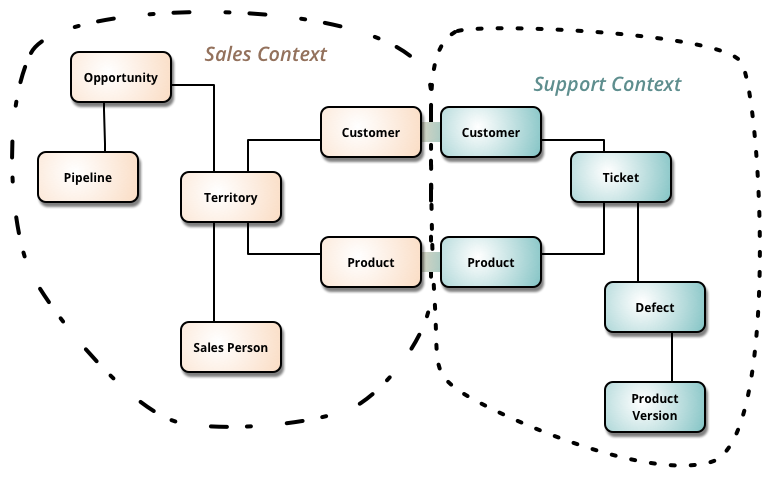
\includegraphics[width=\linewidth]{content/images/BoundedContext}\
    \quelle\url{http://martinfowler.com/bliki/BoundedContext.html}
    \caption[Bounded Context]{Bounded Context\\}
    \label{fig:BoundedContext}  
\end{figure} 
In dieser Grafik wird noch einmal der Begriff Bounded Context genauer verdeutlicht. Es existieren zwei eigenständige Prozesse. Auf der linken Seite der Sales Kontext und auf der rechten Seite der Support Kontext. Jeder Kontext besitzt verschiedene Services, welche benötigt werden um den Prozess durchführen zu können. Lediglich zwischen den \textit{Customer} und \textit{Product} Services besteht eine Verbindung der beiden Prozesse.

\subsection{Das Gesetzt von Conway}
\label{subsec:conway}
Spricht man von "`Service-orientierten Architekturen"', sollte das \glqq Gesetzt von Conway\grqq\ nicht fehlen, da es Prinzipien beschreibt, nach denen eine Unternehmens-Architektur entworfen wird.
\\\\
Melvin Conway ist ein amerikanischer Informatiker und formulierte seine Beobachtungen bezüglich der Kommunikationsstrukturen und Organisationen innerhalb eines Unternehmens. Seine Beobachtung, auch \glqq Gesetzt von Conway\grqq\ genannt lautet wie folgt:
\begin{center}
    \textit{Organisationen, die Systeme designen, können nur solche Designs entwerfen, welche die Kommunikationsstruktur dieser Organisationen abbilden.}
\end{center}

Conway möchte damit ausdrücken, dass die internen Kommunikationswege wichtig bei der Planung der Architektur ist. Jedes Team innerhalb einer Organisation trägt zu der Entwicklung der Architektur bei. Wird eine Schnittstelle zwischen zwei Teams benötigt, so müssen diese Teams auch kommunizieren können. Dabei müssen Kommunikationswege nicht immer offiziell sein. Oft gibt es informelle Kommunikationsstrukturen, die ebenfalls in diesem Kontext betrachtet werden können.
\\\\
Service-orientierte Systeme arbeiten nach dem gleichen Prinzip. Dienste in diesen Systemen sind eigenständig und müssen, damit daraus eine funktionierende Anwendung bzw. System wird, unter einander problemlos kommunizieren können.

\section{Kommunikation: Orchestration vs Choreographie}
\label{sec:OrchestrationVsChoregraphie}

\subsection*{Orchestration}
\label{subsec:orchestration}
Bei der Orchestration handelt es sich um eine Komposition von Services. Ein Geschäftsprozess wird zwar mit Hilfe von mehreren Services abgebildet, jedoch ist nur ein Service dafür zuständig den Geschäftsprozess durchzuführen.
\newpage
\begin{figure}[htb]
    \centering 
    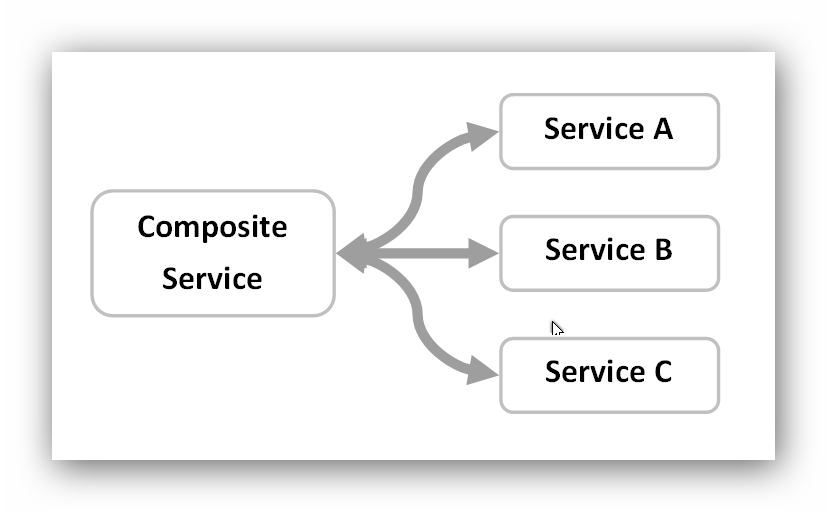
\includegraphics[width=\linewidth]{content/images/ServiceOrchestration}\
    \caption[Orchestration]{Orchestration}
    \label{fig:ServiceOrchestration}  
\end{figure}

Wie die Abbildung \ref{fig:ServiceOrchestration} zeigt besteht bei der Orchestration \textbf{\underline{keine}} Verbindung zwischen:
\begin{itemize}
    \item A \& B
    \item A \& C
    \item B \& C
\end{itemize}
Nur der "`Composite Service"' nutzt die anderen Services, um den Geschäftsprozess abzubilden.

\subsection*{Choreographie}
\label{subsec:choreographie}
Anders als bei der Orchestration können Services bei der Choreographie beliebig untereinander kommunizieren. Das ist sinnvoll, wenn verschiedene Dienste, sich untereinander über Änderungen oder andere Aktionen informieren müssen.
\newpage
\begin{figure}[htb]
    \centering 
    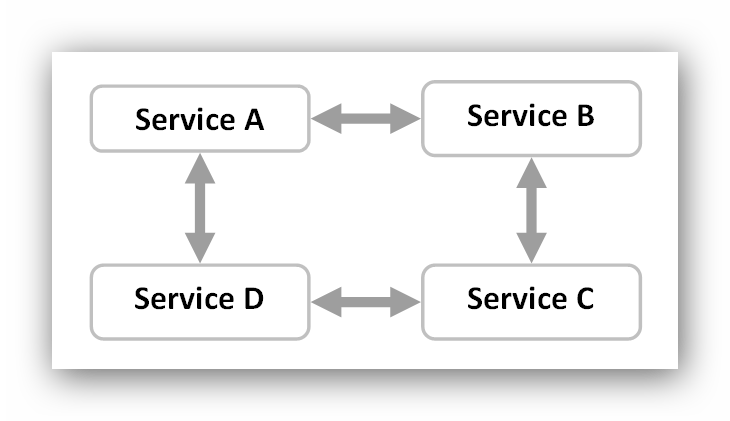
\includegraphics[width=\linewidth]{content/images/ServiceChoreography}\
    \caption[Choreographie]{Choreographie}
    \label{fig:ServiceChoreography}  
\end{figure}
So ist, wie in Abbildung \ref{fig:ServiceChoreography} zu erkennen, eine beliebige Kommunikation zwischen den einzelnen Diensten möglich.

\section{Abgrenzung von monolithischen Systemen}
\label{sec:AbgrenzungVonMonolithischenSystemen}
Im Vergleich zu monolithischen Systemen, muss bei dem Einsatz von Service-orientierten Systemen einiges beachtet werden. So ist die Kommunikation ein wichtiger Faktor. Man muss sich nicht nur zwischen einer der beiden zuvor genannten Kommunikationsformen, Choreographie oder Orchestrierung, entscheiden, es muss zudem sichergestellt werden, dass Nachrichten zugestellt werden.
\\\\
Während bei einem monolithischen System alle Abhängigkeiten innerhalb der Anwendung zu finden sind, besteht die Anwendung in einem Service-orientieren System aus mehreren Diensten, welche untereinander kommunizieren. Jeder Dienst bildet dabei einen gewissen Context ab (siehe \nameref{sec:boundedContext}). Zudem ist es dadurch möglich, dass jeder Dienst eine eigene Datenbank hat, wodurch verschiedene Datenbanksysteme (SQL und NoSQL) eingesetzt werden können. In der nachfolgenden Abbildung ist einem Monolithen, ein Microservice System entgegen gesetzt.
\begin{figure}[htb]
    \centering 
    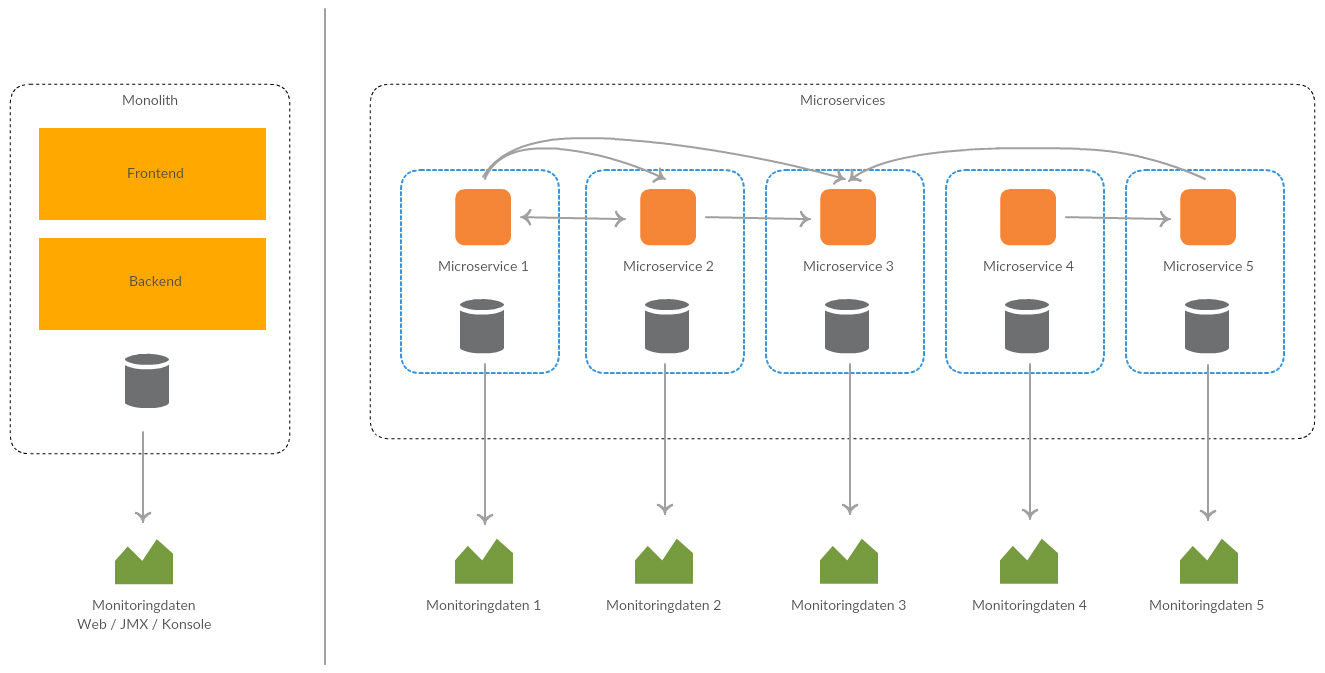
\includegraphics[width=\linewidth]{content/images/fichtner_microservices_1}\
    \quelle\url{https://jaxenter.de/wp-content/uploads/2016/10/fichtner_microservices_1.jpg}
    \caption{Monolithisches vs Service-orientiertes System}
    \label{fig:BoundedContext}  
\end{figure}
Zusätzlich zu den oben genannten unterschieden, sieht man in der Abbildung außerdem ein Monitoring-System. Während bei einem Monolithen, nur ein Monitoring-System benötigt wird, muss bei einem Service-orientiertem System, jeder Service ein Monitoring-System besitzen. Bei großen Systemen, müssen zudem die Monitoring-Informationen gebündelt werden und zentral einsehbar sein.

\chapter{SOA}
\label{chap:soa}
Der Begriff SOA ist nicht eindeutig definiert. Je nachdem welche Person man in einem Unternehmen befragt, erhält man unter Umständen eine komplett andere Definition. \frqq Die meisten Definitionen stimmen jedoch zum größten Teil überein und stehen nicht im Konflikt mit einander.\flqq\ \ \cite[vgl. Seite 6]{100QA}

Für einen Kaufmann ist SOA etwas Anderes als für einen Analysten. Um die unterschiedlichen Sichten auf SOA besser zu verstehen, werden zunächst einmal einige Definitionen nach \cite{100QA}\ genannt:
\begin{enumerate}
       \item \frqq To the chief information officer (CIO), SOA is a journey that
       promises to reduce the lifetime cost of the application portfolio [...].\flqq\  \cite[vgl. Seite 6]{100QA}
    
       \item \frqq To the business executive, SOA is a set of services that can be exposed to their customers, partners, and other parts of the organization. Business capabilities, function, and business logic can be combined and recombined to serve the needs of the business now and tomorrow. Applications serve the business because they are composed
       of services that can be quickly modified or redeployed in new
       business contexts, allowing the business to quickly respond to changing
       customer needs, business opportunities, and market conditions.\flqq\  \cite[vgl. Seite 6]{100QA}
       
       \item \frqq To the business analyst, SOA is a way of unlocking value, because business processes are no longer locked in application silos. Applications no longer operate as inhibitors to changing business needs.\flqq\  \cite[vgl. Seite 6]{100QA}
       
       \item \frqq To the chief architect or enterprise architect, SOA is a means to
       create dynamic, highly configurable and collaborative applications
       built for change. SOA reduces IT complexity and rigidity. SOA becomes the solution to stop the gradual entropy that makes applications
       brittle and difficult to change. SOA reduces lead times and costs
       because reduced complexity makes modifying and testing applications
       easier when they are structured using services.\flqq\  \cite[vgl. Seite 6]{100QA}
\end{enumerate}
Jeder der genannten Rollen hat eine eigene Definition von dem was SOA ist. Jede der Definitionen ist jedoch nur ein Teil dessen für was SOA verwendet werden kann, denn SOA ist ein Paradigma und kein festes Modell. Es dient zur Orientierung, gibt jedoch keine feste Richtung vor. Dabei ist das Ziel von SOA nicht die Entwicklung zu vereinfachen oder voran zu bringen, sondern die unternehmensweiten Geschäftsprozesse zu standardisieren und vereinheitlichen.

\section{Business und IT}
\label{sec:BusinessAndIT}
IT darf nie zum Selbstzweck existieren. Sie wird immer zur Unterstützung der Geschäftsprozesse eingesetzt. Oft existieren bereits verschiedene kommerzielle Systeme und Eigenentwicklungen. Mit SOA soll dafür gesorgt werden, dass diese Systeme möglichst effizient miteinander arbeiten können.
\begin{quotation}
    \frqq The complexity of the technology infrastructure at many companies in the financial services sector makes it very hard to leverage IT services in a coordinated way across the enterprise. Many large companies have either merged or acquired other very large companies resulting in the integration of new business units with very different work cultures and widely different information infrastructurse. The need to be able to trust and understand the information about the business across its many disaggregated parts has been a prime motivator for change in the IT infrastructure at these companies.\flqq\  \cite[S. 17]{SOAForDummies}
\end{quotation}

Mit SOA wird die IT-Infrastruktur eines Unternehmens in zwei Teile geteilt. Auf der einen Seite existiert die Geschäftsschicht mit der Geschäftslogik und auf der anderen Seite die IT-Schicht, welche die Computing-Ressourcen verwaltet. Durch diesen Aufbau ist es nicht nötig, dass ein Business Manager die IT-Schicht verstehen muss.
\\\
In der Geschäftsschicht sind nur Dienste, mit denen Kunden, Lieferanten und Business Partner interagieren. Diese Personen benötigen, genauso wie ein Business Manager, kein Wissen darüber, was in der IT-Schicht existiert oder wie diese aufgebaut ist. Andersherum sind in der IT-Schicht nur Dienste und Applikationen vorhanden, wofür die IT-Abteilung zuständig ist.
\\\\
Damit diese Schichtentrennung funktioniert, wird darauf geachtet, dass in der Geschäftsschicht möglichst wenig Komplexität nach außen sichtbar ist.

\section{Unternehmenskomponenten}
\label{sec:UnternehmensKomponenten}
Unternehmenskomponenten sind ein zentraler Bestandteil von SOA. Die Informationen aus den Komponenten, müssen durch APIs abgerufen werden können. Dienste in einem SOA-System sind nicht, wie anzunehmen, die Unternehmensanwendungen selber, sondern Adapter, welche für die Steuerung der jeweiligen Anwendungen verantwortlich sind. Dabei dient der Adapter nicht nur als \gls{glos:APIExposureGateway}, sondern sorgt auch dafür, dass keine fehlerhaften Anfragen an das System geschickt werden. Spricht man bei SOA von Diensten, ist meistens der Adapter, zusammen mit den Unternehmenskomponenten gemeint. Wird der Begriff "`Dienst"' im Zusammenhang mit SOA verwendet, ist damit der Adapter und die Anwendung bzw. Unternehmenskomponente gemeint.

\begin{quotation}
	\frqq Die SOA-Services werden nicht neu implementiert, sondern sind schon in den Anwendungen im Unternehmen vorhanden. Eine SOA-Einführung macht diese Services außerhalb der Anwendungen verfügbar. Durch die Aufteilung der Anwendungen in Services wird deren Nutzung in verschiedenen Zusammenhängen ermöglicht. [..] Auf Basis der einzelnen Services ist es möglich, Geschäftsprozesse abzubilden und dabei die Services wiederzuverwenden. Dazu ist nur eine Orchestrierung der einzelnen Services notwendig.\flqq\ \cite[S. 84]{EWolff2016:Microservices}
\end{quotation}

Damit die Geschäftsprozesse mit Hilfe von SOA abgebildet werden können, müssen zunächst einmal die dazu gehörenden Komponenten identifiziert werden.

\begin{figure}[htb]
    \centering 
    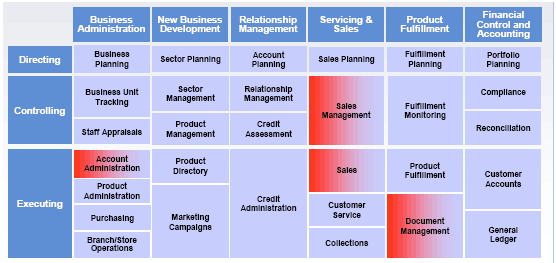
\includegraphics[width=\linewidth]{content/images/UnternehmensKomponenten}\
    \quelle\url{http://www.jot.fm/issues/issue_2008_05/column5/} (Stand 16.12.2016)
    \caption[Unternehmens Komponenten]{Unternehmens Komponenten\\}
    \label{fig:UnternehmensKomponenten}  
\end{figure} 
\newpage
Daraus ergeben sich anschließend die Komponenten, welche untereinander kommunizieren müssen. Die in der Abbildung rot dargestellten Komponenten sind schließlich das Resultat aus der Analyse. Hat man die Komponenten über Kommunikationswege verbunden, werden die nächsten Geschäftsprozesse identifiziert. Diese Prozedur wird solange wiederholt, bis alle Komponenten miteinander verbunden sind.

\section{Enterprise-Service Bus - ESB}
\label{sec:esb}
Der Begriff "`Enterprise-Service Bus"' (ESB) wird oft im Zusammenhang mit SOA verwendet. Der ESB ist jedoch kein Teil von SOA, sondern nur ein Mittel, um die Kommunikation zu vereinheitlichen und ein Exposure Gateway bereitzustellen. Der Enterprise-Service Bus dient dabei als Nachrichtenkomponente, welcher die Nachrichten entgegennimmt und an die jeweiligen Empfänger weiterleitet. Es dient ebenfalls als Transformator von Nachrichten, um die Interoperabilität sicherzustellen. Dabei liegen auf der einen Seite des ESB die Services und auf der anderen Seite die Anwendungen.

\begin{figure}[htb]
    \centering 
    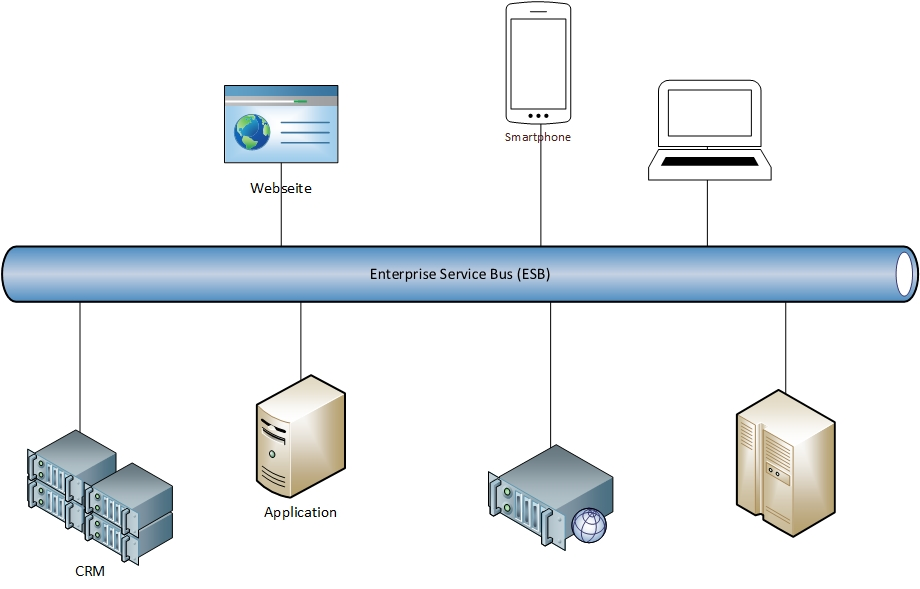
\includegraphics[width=\linewidth]{content/images/ESB}\
    \caption[ESB]{Darstellung einse Enterprise Service Bus, mit Diensten und Frontend Anwendungen}
    \label{fig:esb}  
\end{figure}
\newpage
Dienste bieten eine große Menge an Informationen über deren APIs an. Oft werden jedoch nicht alle Informationen benötigt. Gerade auf mobilen Geräten können viele Daten zu langen Ladezeiten führen. Der ESB filtert und bereitet die Daten der Dienste auf und sendet nur die benötigten Daten. Dadurch werden Anwendungen und Anwender nicht mit unwichtigen Daten überfordert.

\chapter{Microservices}
\label{chap:Microservices}
Ein Microservices-System besteht aus vielen verteilten Anwendungen (Dienste), welche man selber ebenfalls Microservices nennt. Dabei wird versucht, komplexe Anwendungen, in einzelne Dienste aufzuteilen.

\begin{quotation}
    \frqq Modularisierung ist nichts Neues. Schon lange werden große Systeme in kleine Module unterteilt, um Software einfacher zu erstellen, zu verstehen und weiterzuentwickeln. Das Neue: Microservices nutzen als Module einzelne Programme, die als eigene Prozesse laufen. Der Ansatz basiert auf der UNIX-Philosophie. Sie lässt sich auf drei Aspekte reduzieren:\flqq\cite[S. 2]{EWolff2016:Microservices}
\end{quotation}

Weiter nach \cite[S. 2]{EWolff2016:Microservices} haben Microservices folgende Eigenschaften:
\begin{itemize}
    \item Ein Programm soll nur eine Aufgabe erledigen, und das soll es gut machen.
    \item Programme sollen zusammenarbeiten können.
    \item Nutze eine universelle Schnittstelle. In UNIX sind das beispielsweise Textströme.
\end{itemize}

Diese Art der Aufteilung wurde schon lange von großen Unternehmen wie Amazon oder Google genutzt, jedoch fehlte lange Zeit ein Begriff für dieses Paradigma.

\begin{quotation}
    \frqq 2006 hielt Werner Vogels (CTO, Amazon) einen Vortrag auf der JAOO-Konferenz, wo er die Amazon Cloud und Amazons partnermodell vorstellte [1]. Dabei erwähnte er das CAP-Theorem - heute Basis für NoSQL. Und dann sprach er von kleinen Teams, die Services mit eigenener Datenbank entwickeln und auch betreiben. Diese Organisationen nennen wir heute DevOps und die Architektur Microservices.\flqq\ \cite[S. 13]{EWolff2016:Microservices}
\end{quotation}

Der Begriff Microservices ist nicht eindeutig definiert. Als erste Näherung dienen, nach Eberhard Wolff \cite[S. 2]{EWolff2016:Microservices}, folgende Kriterien:

\begin{itemize}
    \item Microservices ist ein Modularisierungskonzept. Sie dienen dazu, ein großes Software-System aufzuteilen - und beeinflussen die Organisation und die Software-Entwicklungsprozesse.
    \item Microservices können unabhängig von Änderungen an anderen Microservices in Produktion gebracht werden.
    \item Microservices können in unterschiedlichen Technologien implementiert sein. Es gibt keine Einschränkung auf eine bestimmte Programmiersprache oder Plattform.
    \item Microservices haben einen eigenen Datenhaushalt: eine eigene Datenbank - oder ein vollständig getrenntes Schema in einer gemeinsamen Datenbank.
    \item Microservices können eigene Unterstützungsdienste mitbringen, beispielsweise eine Suchmaschine oder eine spezielle Datenbank. Natürlich gibt es eine gemeinsame Basis für alle Microservices - beispielsweise die Ausführung virtueller Maschinen.
    \item Microservices sind eigenständige Prozesse - oder virtuelle Maschinen, um auch die Unterstützungsdienste mitzubringen.
    \item Dementsprechend müssen Microservices über das Netzwerk kommunizieren. Dazu nutzen Microservices Protokolle, die lose Kopplung unterstützen. Das kann beispielsweise REST sein - oder Messaging-Lösungen.
\end{itemize}

Grundsätzlich kann man daher Microservices in drei Kategorien einteilen:
\begin{description}
    \item[Producer] Ein Service der etwas produziert oder auf eine Anfrage reagiert. Das reicht von Daten aus einer Datenbank zu extrahieren bis hin zu komplexen Berechnungen.
    \item[Consumer] Ein Service oder eine Anwendung, welche einen oder mehrere produzierende Services verwendet und entweder weiterverarbeitet oder ausgibt. Im Falle der Weiterverarbeitung ist ein Consumer ebenfalls ein Producer.
    \item[Self-Contained System (SCS)] \frqq "`Microservice mit UI"' oder "'Self-Contained System"' wie es Stefan Tilkov nennt, sind in sich abgeschlossene Systeme. [..] Sie enthalten eine UI und sollten möglichst nicht mit anderen SCS kommunizieren.\flqq \cite[vgl S. 55]{EWolff2016:Microservices}.
\end{description}

Ein Self-Contained System ist die optimale Form eines Microservices, da keine weiteren Microservices benötigt werden, um die eigenen Daten darzustellen. Dadurch werden keine anderen Services vorausgesetzt und eine lose Kopplung der Dienste ist möglich.

\section{Aufbau von Microservices}
\label{sec:Aufbau}
Wie bereits erwähnt, sind Microservices eigenständige Dienste. Sie müssen so gebaut sein, dass sie möglichst ohne Abhängigkeiten funktionieren. Um das zu realisieren dürfen Microservices nur lose gekoppelt sein. Damit ist gemeint, dass der Dienst seine Aufgabe selbständig erledigen kann ohne weiter Dienste in Anspruch zu nehmen. Bei "`Self-Contained Systems"' ist ebenfalls eine UI vorhanden. Damit ist das System in sich abgeschlossen und stellt  alle nötigen Eigenschaften bereit, welche für die Darstellung von Informationen benötigt werden. Müssen jedoch andere Dienste verwendet werden, sollte darauf geachtet werden, dass diese austauschbar bleiben und nicht fest mit miteinander verbunden sind. Ist ein Dienst fest mit einem anderen verbunden, sollte die Notwendigkeit des Dienstes infrage gestellt werden.
\\\\
Produzierende Dienste sind meistens auf der untersten Ebene des Systems zu finden und stellen Dienste mit, in sich abgeschlossenen, Aufgaben dar. Konsumierende Dienste sind in der darüber liegenden Schicht zu finden. Sie wird meistens als Middleware verwendet, um Informationen zu aggregieren, zusammenzuführen oder aufzubereiten.
\\\\
Damit ein Dienst selbständig bleibt, besitzt dieser alle dafür notwendigen Ressourcen. Hierzu zählt, unter anderem, eine eigene Datenbank. Dadurch kann das Schema der Datenbank frei verändert werden, ohne, dass weitere Teile des Systems beeinflusst werden. Es ist jedoch darauf zu achten, dass die Schnittstelle des Dienstes, worüber dieser von anderen Diensten ansprechbar ist, nicht grundlegend verändert werden oder die Dienste, welche diese Schnittstelle verwenden, ebenfalls geändert werden. Letzteres ist beispielsweise der Fall, wenn sich Fachlichkeiten des Systemes ändern, da diese in einigen Fällen, über mehrere Microservices verteilt sind. Jedoch besteht hierbei weiterhin die Gefahr, dass einzelne Dienste, die Schnittstelle nutzen, um einzelne Informationen abzurufen, jedoch nichts mit den Fachlichkeiten zu tun hat. In diesem Fall ist zu beachten, dass die Schnittstelle weiterhin das liefert, was zu erwarten ist.
\\\\
Geht man von \textit{Self-Contained Systems} aus, besitzen Microservices zusätzlich noch eigene UI-Elemente. Dadurch kann der Microservice, seine Informationen selber darstellen und damit bestimmen, wie diese dargestellt werden.

\begin{figure}[htb]
	\centering 
	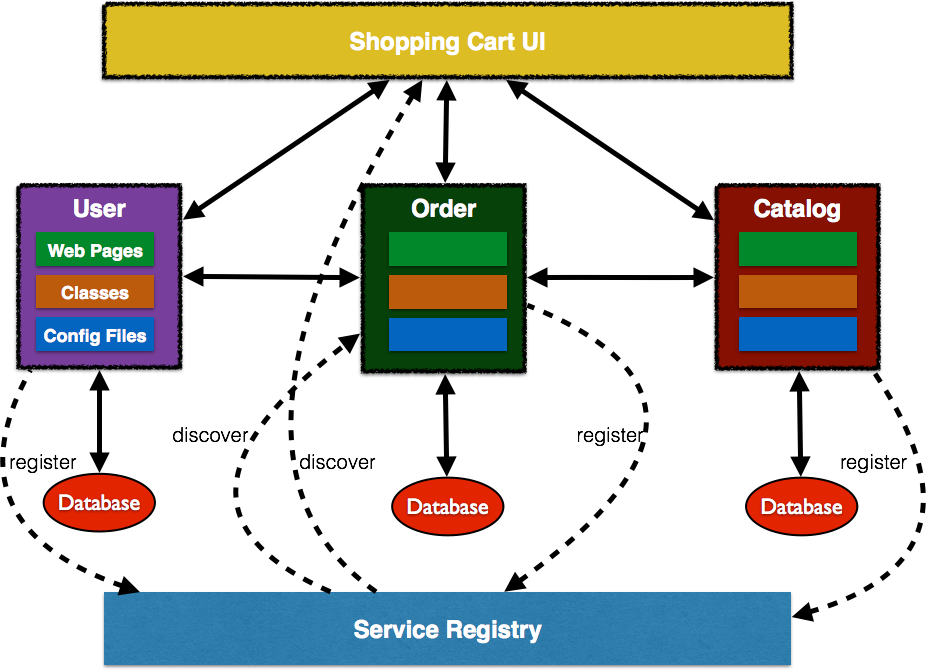
\includegraphics[width=\linewidth]{content/images/javaee-microservices}\
	\quelle\url{http://blog.arungupta.me/monolithic-microservices-refactoring-javaee-applications/} (Stand 16.12.2016)
	\caption{Beispiel einer Microservice Architektur einer Shopping Anwendung}
	\label{fig:MicroserviceArchitektur} 
\end{figure}

\section{Gr"o\ss e von Microservices}
\label{sec:groesseMicroservice}
\begin{quotation}
    \frqq Der Name "`Microservices"' verrät schon, dass es um die Servicegröße geht - offensichtlich sollen die Services klein sein.\flqq\ \cite[S. 31]{EWolff2016:Microservices}
\end{quotation}
Es gibt verschiedene Möglichkeiten die Größe von Programmen zu ermitteln. Eine Variante ist zum Beispiel das Zählen von  Lines of Code (LOC), jedoch hat diese Methode auch Nachteile.

\begin{quotation}
	\frqq Er hängt von der verwendeten Programmiersprache ab. Einige Sprachen benötigen mehr Code, um dasselbe auszudrücken - und Microservices sollen gerade nicht den Technologie-Stack fest definieren. Dementsprechend ist eine Definition anhand dieser Metrik kaum sinnvoll.\flqq\ \cite[S. 31]{EWolff2016:Microservices}
\end{quotation}

Die Größe von Services sollte jedoch nicht von zentraler Bedeutung sein, denn eine untere Grenze gibt es für Services nicht.

\begin{quotation}
    \frqq Wohl aber eine obere Grenze: Wenn der Microservice so groß ist, dass er von einem Team nicht mehr weiterentwickelt werden kann, ist sie zu groß. Ein Team sollte dabei eine Größe haben, wie sie für agile Prozesse besonders gut funktioniert. Das sind typischerweise drei bis neun Personen. Also darf ein Microservice auf keinen Fall so groß werden, dass ein Team ihn nicht mehr alleine weiterentwickeln kann.\flqq\ \cite[S. 33f]{EWolff2016:Microservices}
\end{quotation}

Bei der Größe eines Services ist darauf zu achten, dass ein Service nicht zu viele oder zu wenige Funktionen besitzt. Wie bereits beschrieben, sind Microservices modulare, lose gekoppelte Services. Wird ein Service zu klein angesetzt, können daraus Abhängigkeiten zu anderen Services entstehen und damit das Gesetzt der losen Kopplung verletzten. Besitzt hingegen ein Service zu viele Funktionen, wird es meistens nicht mehr als Microservice angesehen, da dadurch der Microservice mehr als eine Aufgabe übernimmt.

\section{Orchestration vs Choreographie}
\label{sec:orchestrationvschoreographie}
Möchte man ein Microservice System aufbauen, stellt sich die Frage, wie einzelne Services strukturiert werden und wie diese untereinander kommunizieren sollen. Ein bestimmter Vorgang startet in der Regel bei einem Service. Nun muss entschieden werden, ob weitere Services hinzugezogen, beziehungsweise informiert werden müssen.
Je nach Anwendungsfall muss man sich zwischen Service Orchestration und Choreographie entscheiden. Dabei ist es fast unmöglich ein ganzes Microservice-System aus nur einem der beiden Varianten zu bauen.

% [Seite 66 EWolff2016] Technologische Wahlfreiheit
\subsection{Herausforderung}
\label{sec:Herausforderung}
Der Ausfall eines Services kann im schlechtesten Fall dazu führen, dass alle anderen Microservices nicht mehr funktionieren. Um das zu verhindern muss klar definiert werden, was Microservices in dieser Situation tun sollen. Zusätzlich muss, sofern Datenbankoperationen eine wichtige Rolle spielen, das Problem der einheitlichen Transaktion gelöst werden. Wenn zum Beispiel eine Operation Daten über verschiedene Microservices in Datenbanken schreibt, muss bei nicht Erreichbarkeit oder dem Auftreten eines Fehlers in einem Microservices ein einheitliches Rollback durchgeführt werden, um keine inkonsistenten Daten im System zu erzeugen.

\begin{quotation}
    \frqq Transaktion haben die ACID-Eigenschaften. [..] Innerhalb eines Microservice können Änderungen in einer Transaktion stattfinden. Ebenso kann die Konsistenz der Daten in einem Microservice sehr einfach garantiert werden. Über einen Microservice hinaus wird das schwierig. Dann ist eine übergreifende Koordination notwendig. Bei einem Zurückrollen einer Transaktion müssten alle Änderungen in allen Microservices rückgängig gemacht werden.\flqq\ \cite[S. 35]{EWolff2016:Microservices}
\end{quotation}

Daneben muss sichergestellt werden, dass Nachrichten erfolgreich verarbeitet werden und auch bei mehrfachen senden einer Nachricht darf keine Fehler auftreten. Dafür müssen Microservices Idempotent sein. Das heißt, dass eine wiederholte Aktion (mit gleichen Daten) nicht zu unterschiedlichen Resultaten führt. Wird keine Idempotenz sichergestellt, kann dies zu unerwarteten und unerwünschten Ereignissen führen.
\\\\
Eine weitere Herausforderung besteht in dem Grundkonzept von Microservices. Da nicht definiert ist, welche Programmiersprache für Microservices verwendet wird, kann ein Service zum Beispiel in Java, ein anderes in Scala oder Python geschrieben werden. Es muss daher dafür gesorgt werden, dass die einzelnen Services untereinander interoperabel sind. Um das zu gewährleisten, müssen die Schnittstellen möglichst einheitlich und auf dem gleichen Protokoll aufbauend programmiert werden. Hier bieten REST-Schnittstellen eine gute Lösung. Diese beruhen auf dem HTTP-Protokoll. Zusätzlich bietet das HTTP-Protokoll die Möglichkeit, ein einheitliches Medium, wie zum Beispiel XML oder JSON, als Informationsträger zu nutzen. Dabei kann theoretisch jeder Microservice mit jedem anderen Microservice kommunizieren, sofern die Schnittstellen einheitlich definiert sind.
\\\\
Damit die Schnittstellen genutzt werden können, müssen die Kommunikationskanäle dafür existieren. Nach dem Gesetz von Conway, bedeutet dies, dass die einzelnen Abteilungen bzw. Teams die nötigen Kanäle dafür schaffen müssen.

\begin{figure}[htb]
	\centering 
	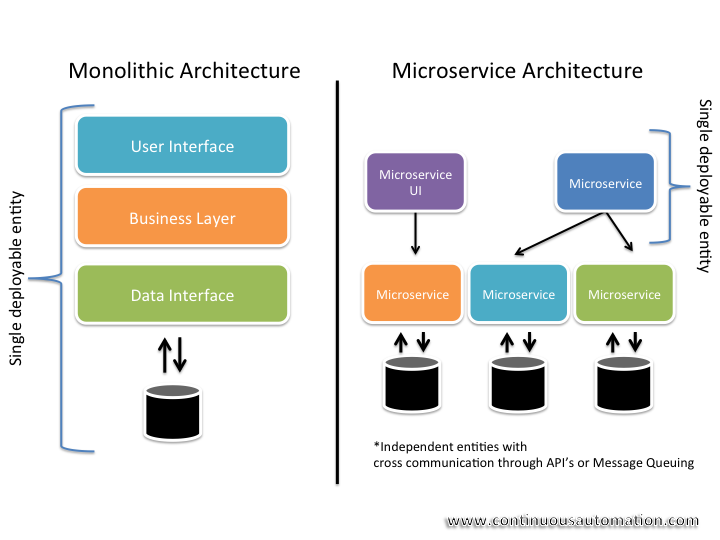
\includegraphics[width=\linewidth]{content/images/570495-slide1}\
	\quelle\url{https://dzone.com/articles/scalable-cloud-computing-with-microservices} (Stand 16.12.2016)
	\caption{Monolithisch vs Microservice Architektur\\}
	\label{fig:MonoVSMicroArchitektur} 
\end{figure}
\newpage
Im Unterschied zu monolithischen Anwendungen, bei der alles in einer Anwendung ist, sind Microservices Module eines gesamten Systems und werden von den jeweiligen Teams entwickelt und verwaltet. Wird eine neue Funktion benötigt, welche nicht in der eigenen Fachlichkeit liegt, muss das entsprechende Team damit beauftragt werden, diese zu implementieren, bzw. in einem bestehenden Microservice anzupassen.

\section{PUSH- VS PULL-Architektur}
\label{sec:PushPullArchitektur}
Grundlegend können Microservices mit Hilfe zwei verschiedener Kommunikations-Architekturen kommunizieren, PUSH- und PULL-Architektur. Dabei ist jedoch nicht ausgeschlossen, dass sobald eine Architektur gewählt worden ist, die andere nicht mehr genutzt werden kann. Genauso wie bei der Entscheidung über die Kommunikationsstruktur (siehe \ref{subsec:orchestration} \nameref{subsec:orchestration}), kann es von Vorteil sein, beide Architekturen zu nutzen.
\\\\
\textbf{PULL-Architektur}\\
Eine PULL-Architektur basiert auf einen einfachen Request-Replay-Schema. Dementsprechend ist das Web PULL-basiert.
Der Browser macht eine Anfrage an einen Server, dieser wiederum verarbeitet die Anfrage und liefert eine Antwort (Replay) zurück. Dies hat den Vorteil, dass nicht lange auf eine Antwort gewartet werden muss und sich die teilhabenden Kommunikationspartner gegenseitig kennen. Ein Nachteil jedoch ist es, dass dadurch weitgehend eine synchrone Kommunikation stattfindet und eine Antwort häufig nicht gleichzeitig an mehrere Empfänger senden kann.
\\\\
\textbf{PUSH-Architektur}\\
Eine PUSH-Architektur wird eingesetzt, wenn man verschiedene Kommunikationspartner über bestimmte Ereignisse informieren möchte oder eine Rückantwort ist nicht erforderlich. Zum Beispiel muss eine Registrierung in unserem fiktiven Unternehmen möglich sein. Dabei sendet der Microservice der für die Registrierung zuständig ist eine einfache Event-Nachricht, wie Benutzer XY hat sich Registriert. Im Hintergrund erhalten anderer Microservices diese Nachricht und führen zusätzliche Aktionen durch, wie das Erstellen des Warenkorbs oder das Anlegen des Profils.
\\\\
Bei der PUSH-Architektur stehen meist nicht die Kommunikationspartner, sondern die Informationen im Vordergrund. Dafür wird meistens ein eigenständiger Service (Broadcaster) eingesetzt, der die Verteilung dieser Informationen übernimmt. Dabei kann ein Service als Informationsprovider dienen, zum Beispiel ein Nachrichten-Feed (von einer Nachrichtenseite). Alle anderen Services abonnieren den Broadcaster und erhalten dadurch alle Nachrichten, die der Informationsprovider sendet.
\\\\
Es gibt jedoch auch den Fall, dass die Kommunikation sternförmig um den Broadcaster angeordnet ist. Dadurch ist jeder Service der diesen abonniert, sowohl Provider, als auch Consumer. Anders als bei PULL-basierten Systemen kann hier nicht durchgehend sichergestellt werden, dass alle Nachrichten von allen Konsumenten gleichzeitig gelesen und ggf. verarbeitet werden. Jedoch können so Informationen innerhalb eines Microservice-Systems relativ zuverlässig verteilt werden.
\\\\
Der Vorteil von PUSH-Architekturen ist, dass eine asynchrone Informationsverbreitung aufgebaut werden kann. Zudem können Serviceausfälle, solange es nicht der Broadcaster oder wichtige Microservices sind, überbrückt werden, indem der Broadcaster die Nachrichten für eine bestimmte Zeit vorhält. Dadurch kann ein ausgefallener Microservice, die Nachricht zu einem späteren Zeitpunkt entgegennehmen und verarbeiten.

\chapter[Gemeinsamkeiten und Unterschiede]{Gemeinsamkeiten und Unterschiede von SOA und Microservices}
\label{chap:Unterschiede}
%Einsatzmöglichkeiten!!!! 
% - nötigen Architekturen und Schnittstellen 
% - Plattformen und Voraussetzungen für den Einsatz der jeweiligen Paradigmen

%Vor- und Nachteile der Paradigmen, 
% - Prozessisolierung
% - Skalierung
% - Deployment
% - Wartbarkeit (insbesondere der Korrigierbarkeit, Erweiterbarkeit, Anpassbarkeit, Verbesserung)
% - Entwicklung/Testbarkeit 
% - Bindung an Technologiestacks
\section{Einsatzgebiet}
\label{sec:Einsatzgebiet}
Sowohl SOA, als auch das Microservice sind Paradigmen aus der Service-orientierten Architektur, verfolgen jedoch unterschiedliche Ansätze. Während das Microservice-Paradigma die Softwareentwicklungsabteilung unterstützen soll, soll mit Hilfe von SOA die Kommunikation zwischen den Anwendungen und den Abteilungen standardisiert und optimiert werden.
\\\\
Mit Hilfe des Microservice Paradigmas wird die Struktur einer Anwendung in mehrere, kleinere Dienste aufgeteilt. Dadurch ist es möglich neue Technologien einzusetzen und gegebenenfalls zu ersetzten, sollten diese nicht den gewünschten Erfolg bringen.
\\\\
Anders sieht es jedoch mit SOA aus. Hierbei werden Adapter für Anwendungen, wie ERP-, CRM- oder COBAL-Systeme, entwickelt, welche zusammen mit der Anwendung als Dienst dienen. Der Adapter stellt eine Schnittstelle für die Funktionalität der Anwendung bereit und übernimmt das steuern der Anwendung und das abfangen von Fehleingaben.

\section{Architekturen und Schnittstellen}
\label{sec:ArchitekturenUndSchnittstellen}
Beide Paradigmen sind Service-orientierte Systeme, dessen Grundlage ein verteiltes System ist. Dabei existieren eine beliebige Anzahl verschiedener Dienste, welche verschiedene Funktionalitäten bereitstellen. Damit der Ausfall eines Dienstes, keine weiteren Dienste direkt beeinflusst, werden diese oft in eigenen Umgebungen betrieben, wie Virtuelle Maschinen. Dies ist sowohl bei SOA, als auch bei Microservices der Fall, jedoch kann durch den Ausfall eines Dienstes die Kommunikation von anderen Diensten gestört werden.
\\\\
Während bei SOA eine zentrale Kommunikationseinheit (der ESB) existiert, sind Microservices in der Kommunikation frei. Dies bedeutet, dass der ESB in einem SOA-System entsprechende Werte oder Fehlermeldungen zurückgeben kann, während Microservices selber auf fehlgeschlagene Anfragen reagieren muss. Um dies zu verhindern, werden oft mehrere Instanzen eines kritischen Dienstes betrieben.
\\\\
Damit Dienste untereinander kommunizieren können, sind Schnittstellen (APIs) notwendig, über welche die Informationen abgefragt bzw. bereitgestellt werden können. Da jedoch in einem SOA-System ganze Applikationen wie CRM- oder COBOL-Systeme verwendet werden, ist es notwendig zunächst einmal zu entscheiden, wie dessen Funktionalitäten angeboten werden sollen.
\\\\
Zum einen können Adapter verwendet werden, die jegliche Informationen der Anwendung bereitstellen. Dadurch ist es möglich durch Standardisierte Verfahren wie SOAP/HTTP oder REST/HTTP den Dienst wiederzuverwenden. Jedoch muss dafür neben den Adaptern ein Integrations Hub (ESB) existieren, welche die Informationen verarbeiten und aufbereiten kann. 
\\\\
Zum anderen bedeutet diese Aufteilung, dass oft eine große Menge an Informationen abgefragt werden. Dies macht gegenüber dem Business kein Sinn, da zum Teil unnötig viele Informationen für die nächste Generation von Anwendungen bereitgestellt werden. In diesem Fall werden "`Service Komponenten"' verwendet, welche als Adapter dienen und die benötigten Informationen aus den Applikationen abfragen und bereitstellen.
\begin{figure}[htb]
    \centering 
    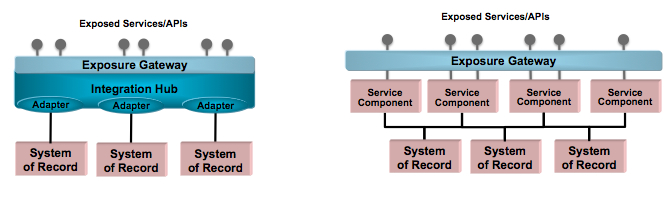
\includegraphics[width=\linewidth]{content/images/figure2}\
    \quelle\url{https://www.ibm.com/developerworks/websphere/library/techarticles/1601_clark-trs/1601_clark.html}
    \caption{Technische und Funktionale Sicht von SOA}
    \label{fig:TechnicalAndFunctionalViewsOfSOA} 
\end{figure}

Bei einem Microservice System stellt ein Microservice genau eine Fachlichkeit da und bietet diese über Schnittstellen an. Anders als bei SOA sind die Dienste deutlich kleiner, wodurch weniger Informationen bereitgestellt werden, je Microservice.
\begin{figure}[htb]
    \centering 
    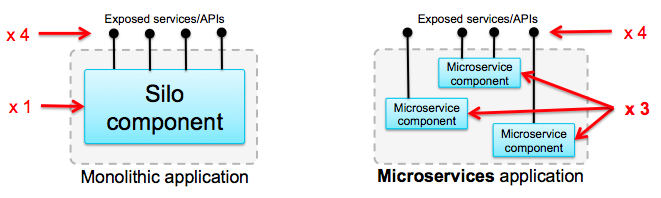
\includegraphics[width=\linewidth]{content/images/MonolithicVsMicroservice}\
    \quelle\url{https://www.ibm.com/developerworks/websphere/library/techarticles/1601_clark-trs/1601_clark.html}
    \caption{Monolithische vs Microservice Applikation}
    \label{fig:MonolithicVsMicroservice} 
\end{figure}
\newpage
Dies bedeutet jedoch auch, dass weitere Microservices notwendig sind, welche die Informationen von verschiedenen Microservices abfragen und zusammenfassen. Dadurch ergibt sich ein Geflecht aus Microservices, welche untereinander kommunizieren und zum Teil aufeinander angewiesen sind. Solange sich die Schnittstelle eines Dienstes nicht ändert, besteht kein Problem bei der Interoperabilität für das bestehende System. Erst wenn sich die Schnittstelle ändert und eine ältere Schnittstelle nicht mehr Angeboten wird, schadet dies der Interoperabilität.
\\\\
Dadurch, dass die Kommunikation über Schnittstellen erfolgt, kann, sofern diese Standardisiert sind und Beispielsweise als SOAP/HTTP oder REST/HTTP umgesetzt wurden, der Dienst Plattform unabhängig deployed werden. Da jedoch monolithische Anwendungen oft sehr umfangreich sind, werden diese meistens für ein bestimmtes Betriebssystem gebaut. Microservices hingegen sind kleine autarke Dienste, Dadurch ist es möglich diese Plattform unabhängig zu deployen. Hier drauf wird in weiter unten, unter \ref{subsec:BindungAnTechnologiestacks} \nameref{subsec:BindungAnTechnologiestacks}, genauer eingegangen.

\section{Vor- und Nachteile}
\label{sec:VorUndNachteile}

\subsection{Prozessisolierung}
\label{subsec:Prozessisiolierung}
Ein wichtiger Grundsatz von Service-orientierten Systemen ist, dass Dienste autark bleiben. Um dies zu erreichen, darf nur eine lose Kopplung zwischen einzelne Dienste stattfinden. Dies wird durch Zustandslose Schnittstellen und Eigenständigkeit erreicht. Damit ist gemeint, dass jeder Dienst seine Aufgaben, zum größten Teil alleine durchführen kann ohne auf andere Dienste angewiesen zu sein.
\\\\
Eine Vollständige Autarkheit ist in einem Microservice System nicht möglich, da ein vollständiges Microservice System die Abbildung einer Applikation ist. Dabei wurden einzelne Fachlichkeiten in Microservices verpackt. Dadurch können einige Microservices nicht lose gekoppelt sein, sondern benötigen weitere Microservices.

\begin{figure}[htb]
    \centering 
    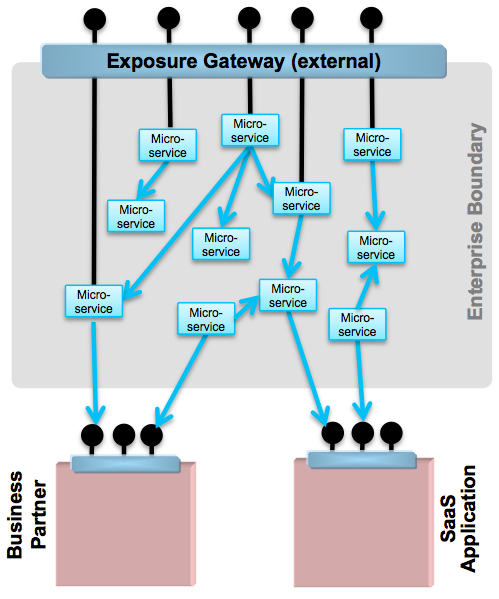
\includegraphics[width=300px]{content/images/figure6}\
    \quelle\url{https://www.ibm.com/developerworks/websphere/library/techarticles/1601_clark-trs/1601_clark.html}
    \caption{Microservice Architektur}
    \label{fig:MicroserviceArchitekturInGreenField} 
\end{figure}
\newpage
Bei SOA hingegen besteht ein Dienst, wie bereits in \ref{sec:UnternehmensKomponenten} \nameref{sec:UnternehmensKomponenten} erwähnt, aus einer vollständigen Anwendung und einem Adapter, welcher die Steuerung der Anwendung über APIs bereitstellt. Dadurch dass eine Anwendung alle nötigen Fachlichkeiten und Ressourcen, für die Ausführung der Anwendung besitzt, ist der Dienst vollständig Autark. Lediglich die Frontend-Anwendungen sind auf die APIs und damit auf die Backend-Anwendungen angewiesen. Fällt zum Beispiel eine Anwendung aus, kann es dazu führen, dass das gesamte System nicht mehr funktioniert, da die Dienste häufig in eine Wertschöpfungskette eingebunden sind.

\subsection{Deployment}
\label{subsec:Deployment}
Das Deployment ist in einem Service-orientiertem System von entscheidender Bedeutung und darf nicht unterschätzt werden. Oft werden Continuous Deployment Pipelines aufgebaut, um diesen Prozess zu automatisieren. Innerhalb der Pipeline wird sowohl die Umgebung, in welcher der Dienst später laufen soll, aufgebaut, sowie der Dienst in die zuvor, vorbereitete Umgebung deployed. Unter Umständen ist ein erneutes Deployen notwendig, wenn sich die Anforderungen an einen Dienst geändert haben oder Fehler behoben wurden. Dabei stellt das Deployment eine besondere Herausforderung dar. Hauptproblem ist die nötigen Abhängigkeiten, für die Ausführung der Dienste, bereitzustellen und die nötigen Konfigurationen vorzunehmen.
\\\\
Dadurch, dass Microservices kleine autarke Dienste sind, ist es oft nicht nötig, viele Konfigurationsdateien anzupassen bzw. bereitzustellen. Jedoch sind oft eine Vielzahl von Microservices in einem System vorhanden und müssen deployed, sowie gemanagt werden. Durch Werkzeuge wie \gls{glos:Docker} und \gls{glos:Vagrant} wird das Deployment zusätzlich vereinfacht. 
\\\\
Dienste in einem SOA-System hingegen sind häufig ganze Anwendungen. Diese erfordern oft eine aufwändige Konfiguration, welche nicht immer mit Hilfe von Konfigurationsdateien vorgenommen werden können. Einige Anwendungen dürfen nur durch den Hersteller oder durch ihn Zertifizierte Unternehmen Installiert und/oder Konfiguriert werden. Dadurch ist ein automatisches Deployment nicht möglich und auch ein manuelles Deployment wird erschwert.
\\\\
Im Rahmen einer Wartung müssen Dienste, oft erneut ausgeliefert werden, um Fehler zu beheben oder ihn anzupassen. In diesem Falle existieren in der Regel die Umgebungen, für den Einsatz des Dienstes. Jedoch müssen diese gegebenenfalls angepasst werden. Die ist in einem Microservice-System durch Werkzeuge wie Docker ebenfalls standardisiert. In einem SOA-System hingegen muss dies oft manuell durchgeführt werden.

\subsection{Skalierung}
\label{subsec:Skalierung}
Nicht immer können stark genutzte Anwendungen, durch Aufwertung oder Erweiterung von Hardware, belastbarer gemacht werden. Kritische oder Zentrale Anwendungen eines Unternehmens sind nicht nur stark genutzt, sondern dürfen nicht ausfallen. Durch Hardware, kann nicht durchgängig sichergestellt werden, dass eine Anwendung erreichbar ist. Um diese Problematiken entgegen zu wirken, muss Skaliert werden. Dabei werden mehrere Instanzen eines Systems parallel betrieben.
\\\\
In einem Microservice-System, ist durch das vereinfachte Deployment möglich, in kürzester Zeit eine weitere Instanz eines Dienstes zu starten und zu betreiben. Dies kann durch einen Standardisierten Deployment Prozess automatisiert werden. Dadurch kann in kürzester Zeit auf verschiedene Lasten von Diensten reagiert werden, ohne dass ein Mensch in das System eingreifen muss. Es ist bei einem Microservice-System möglich, wenig genutzte Dienste, nur bei bedarf zu starten und nach einer gewissen Zeit der Inaktivität, zu stoppen. Kritische oder stark genutzte Dienste hingegen, besitzen meistens mehrere Instanzen, auf denen die Lasten verteilt werden. Dadurch wird ebenfalls eine Ausfallsicherheit gewährleistet.
\\\\
SOA-Systeme besitzen deutlich größere Dienste als Microservice-Systeme. Dadurch dass, wie bereits unter \ref{subsec:Deployment} \nameref{subsec:Deployment} erwähnt, der Deployment Prozess nicht Standardisiert ist, ist ein einfaches, automatisches Skalieren nicht möglich. Das Skalieren eines Dienstes kann dementsprechend, nur manuell geschehen und ist oft mit viel Aufwand verbunden. Muss ein Dienst dennoch mehrere Instanzen besitzen, so werden diese meistens dauerhaft, parallel betrieben.
\\\\
Viele monolithische Anwendungen sind zudem nicht Zustandslos, wodurch ein Skalieren zusätzlich erschwert wird. Microservices hingegen müssen so erstellt werden, dass sie Zustandslos sind, da ein Dienst nicht sicherstellen kann, dass die Anfragen vom gleichen Dienst oder Benutzer stammen.

\subsection{Wartbarkeit}
\label{subsec:Wartbarkeit}
Im laufe der Zeit wachsen die Anforderungen an einen Dienst, wodurch dieser angepasst, verbessert oder erweitert werden muss. Zur Wartung gehört jedoch auch das korrigieren von Fehlern, welches einer der einfachsten Aufgaben in einem Service-orientierten System ist, da sich dadurch meistens, nicht die Schnittstellen, Umgebung oder die Konfiguration des Dienstes ändert. Anders sieht dies jedoch beim anpassen, verbessern oder erweitern aus.
\\\\
Das Anpassen einer Anwendung kann sich von dem Verbessern oder Erweitern einer Anwendung unterscheiden. Zum Beispiel reicht es aus die Mehrwertsteuer in einer Anwendung zu ändern, welches eine Anpassung darstellt, jedoch keine Verbesserung oder Erweiterung. Das Anpassen ist durch die kaum veränderten Strukturen relativ leicht. Anders sieht dies jedoch bei Verbesserungen oder Erweiterungen aus. Beide Änderungen sorgen für eine Veränderung der internen Struktur des Quelltextes. Zusätzlich ist man an den vorgegebenen Technologiestacks gebunden. Oft sind Verbesserungen oder Erweiterungen nicht ohne das Verändern der Quelltextstruktur möglich.
\\\\
Während in einem SOA-System der Dienst aus einer Anwendung und einem Adapter besteht und damit ein fast monolithisches System abbildet. Besteht ein Microservice-System aus viele unterschiedlichen Diensten. In beiden Systemen ist es möglich, in kürzester Zeit Fehler zu korrigieren, sofern die nötigen Voraussetzungen gegeben sind. Das Anpassen, Verbessern oder Erweitern eines Dienstes, gestaltet sich jedoch einfacher in einem Microservice-System, als in einem SOA-System. Aufgrund der Größe von Microservices, kann ein Microservice von Grund auf neu erstellt werden, sollte dies nötig sein. Muss das System erweitert werden, können neue Microservices erstellt, welche die neuen Anforderungen bzw. Fachlichkeiten abbilden. Durch die Autarkheit von Microservices, können diese deployet werden, ohne die Interoperabilität des bestehenden Systems zu gefährden oder zu beeinflussen. Anschließend müssen gegebenenfalls einzelne Dienste angepasst werden, um die neuen Funktionalitäten, in das bestehende System, einzubinden.

\subsection{Bindung an Technologiestacks}
\label{subsec:BindungAnTechnologiestacks}
In beiden Paradigmen, sollten Dienste eine standardisierte Schnittstelle besitzen, damit diese, durch andere Dienste verwendet werden können. Zusätzlich ist dadurch eine Wiederverwendung des Dienstes möglich. Das verwenden einer standardisierten Schnittstelle schränkt jedoch die Auswahl der einzusetzenden Technologien ein. Zudem ist das verwenden einer standardisierten Schnittstelle nicht immer möglich.
\\\\
In einem Microservice-System ist die Wiederverwendbarkeit ein wichtiges Thema. Dadurch wird man gezwungen, die Schnittstellen zu standardisieren. Oft werden hierfür REST-HTTP Schnittstellen, welche Sprachen unabhängig sind, verwendet. REST-HTTP basiert dabei auf dem HTTP-Protokoll. Dadurch kann die Schnittstelle in fast jeder Programmiersprache verwendet werden, wodurch ein Dienst ebenfalls in fast jeder Programmiersprache geschrieben werden kann. Durch die Größe eines Microservices ist es ebenfalls möglich, neue Technologien zu Testen und in der Produktion einzusetzen. Dabei können verschiedenen Sprachen, sowie Frameworks verwendet werden, um die Aufgabe zu erledigen. Stellt sich heraus, dass eine Technologie, Sprache oder Framework sich nicht für die Erledigung einer Aufgabe eignet, kann der Dienst, aufgrund seiner Größe, in kürzester Zeit ausgetauscht werden. Jedoch birgt das einsetzten neuer Technologien auch Gefahren. So ist die Versuchung Groß, experimentelle oder ungetestete Technologien in Produktion einzusetzen, ohne zuvor zu Testen, welche Auswirkungen die Technologie auf das System hat.
\\\\
Ein Dienst in einem SOA-System beinhaltet eine monolithische Anwendung. Die Schnittstellen werden durch Adapter bereitgestellt. Diese müssen mit der Anwendung interagieren können, wodurch der Adapter oft in der selben Sprache geschrieben werden muss, wie die zu interagierenden Anwendung. Aufgrund der Größe von Monolithen ist es nicht möglich, diese in kürzester Zeit auszuwechseln. Zudem muss man sich bei der Entwicklung einer Anwendung, auf einen Technologiestack festlegen. Dadurch ist man bei der Weiterentwicklung oder Wartung der Anwendung an diesen gebunden. Eine neue Technologie einzuführen, würde bedeuten die Struktur der Anwendung zu verändern.

\subsection{Entwicklung und Testbarkeit}
\label{subsec:EntwicklungUndTestbarkeit}
Damit ein Dienst in die jeweiligen Systeme eingebunden werden kann, muss dieser zunächst entwickelt und getestet werden. Dabei ist zu beachten, dass in einem SOA-System, ein Dienst eine monolithische Anwendung mit Adapter ist, während ein Microservice-System eine vollständige Anwendung beschreibt und ein Dienst nur ein Teil der Anwendung ist.
\\\\
Durch diese Unterschiede ist nicht nur die Größe des Entwicklerteams unterschiedlich, sondern auch der Entwicklungsprozess. In einem Microservice-System werden häufig DevOp-Teams in der Größe von 4-6 Personen eingesetzt. Da ein Dienst in einem Microservice-System, nur von einem Team entwickelt werden sollte, stellt dies eine Begrenzung der Größe eines Dienstes dar. Dadurch ist in der Regel ein Microservice deutlich kleiner, als eine monolithische Anwendung, jedoch nicht immer einfacher zu entwickeln.
\\\\
Während bei einer monolithischen Anwendung, alle nötigen Abhängigkeiten in einem Projekt vorhanden sind, muss bei Microservices dafür gesorgt werden, dass die Abhängigkeiten korrekt aufgelöst werden, da diese in dem Bereich anderer Microservices  liegen. Damit die Abhängigkeiten korrekt aufgelöst werden können, muss ein Entwickler wissen, welche Abhängigkeiten die korrektens ind.. In einem Microservice-System gibt es eine sehr große Menge an Diensten, welche verschiedene Fachlichkeiten bereitstellen, daher ist es nicht immer einfach den richtigen Service auszuwählen.
\\\\
Nach der Entwicklung eines Dienstes, muss dieser getestet werden, bevor der Dienst in die Produktion deployed werden kann. In einer monolithischen Anwendung, kann mit Hilfe von automatischen JUnit Tests ein Großteil der Funktionalität getestet werden. Es kann unter anderem getestet werden, ob jegliche Abhängigkeiten innerhalb der Anwendung einwandfrei funktionieren. Benötigt ein Microservice keine anderen Dienste, so kann mit Hilfe von JUnit Tests ebenfalls die Funktionalität vollständig geprüft werden. Anders sieht das jedoch bei Microservices aus, die auf weitere Dienste angewiesen sind. Hierbei müssen entweder die anderen Dienste simuliert werden oder der Microservice muss in eine entsprechende Testumgebung deployed und dort getestet werden. Das betreiben einer solchen Testumgebung ist nicht unproblematisch, da eine exakte Kopie des Produktivsystems notwendig ist, um relevante Testergebnisse zu erlangen.
\\\\
Zudem sollte in jedem der beiden Systeme getestet werden, wie sich einzelne Services, beziehungsweise das gesamte System, bei zufälligen Ausfällen von verschiedenen Systemen, verhalten. Dies stellt eine besondere Herausforderung dar, da dies meistens nur in der Produktionsumgebung möglich ist. Netflix Inc., welches auf Microservices für ihren Dienst "`Netflix"' setzt, hat für diesen Zweck ein Werkzeug Namens "`chaosmonkey"' entwickelt, welches willkürlich Systeme innerhalb seines Dienstes "`Netflix"' abschaltet.\footnote{\cite{chaosmonkey}}


\chapter{Fazit}
\label{chap:Fazit}
Ziel dieser Arbeit war es, die Gemeinsamkeiten und Unterschiede zwischen SOA und Microservices herauszuarbeiten. Dazu wurden die Vor- und Nachteile der beiden Paradigmen hinsichtlich Prozessisolierung, Skalierung, Deployment, Wartbarkeit (Korrigierbarkeit, Erweiterbarkeit, Anpassbarkeit, Verbesserung), Entwicklung/Testbarkeit und die Bindung an Technologie-Stacks analysiert und anschließend verglichen.
\\\\
Nach der Analyse und dem Vergleich der beiden Paradigmen, kann man sagen, dass die Herangehensweise beider Architekturmodelle auf unterschiedlichen Ebenen arbeiten, jedoch das gleiche Ziel verfolgen. Beide Ansätze sollen das Umsetzten neuer Anforderungen vereinfachen.

Bei einem Microservice-System wird dies erreicht, in dem Anwendungen in kleinere Dienste aufgeteilt werden, wodurch die Entwicklung vereinfacht werden soll. Durch die Aufteilung können unterschiedliche Teams an neuen Funktionen arbeiten und deployen, ohne unbedingt auf andere Teams warten zu müssen.

SOA verfolgt hingegen das Ziel, die gesamte Unternehmens-IT zu vereinheitlichen und in einzelne Services aufzuteilen. Dabei wird eine Abstraktionsschicht über den vorhandenen Services eingeführt, um diese neu kombinieren zu können. Damit soll erreicht werden, dass eine flexible Integration der vorhandenen Anwendungen möglich ist und nur die Informationen dargestellt und verarbeitet werden, welche wirklich benötigt werden.
\\\\
SOA und Microservices schließen sich nicht gegenseitig aus. Microservice-Systeme können Teil eines SOA-Systems sein und ihre Aufgaben in diesen einbinden. Dabei wird ein Microservice-System wie eine vollständige Anwendung behandelt. Der  Unterschied ist jedoch, dass meistens deutlich mehr Schnittstellen zur Verfügung gestellt werden können, aufgrund der internen Struktur.
\begin{figure}[htb]
    \centering 
    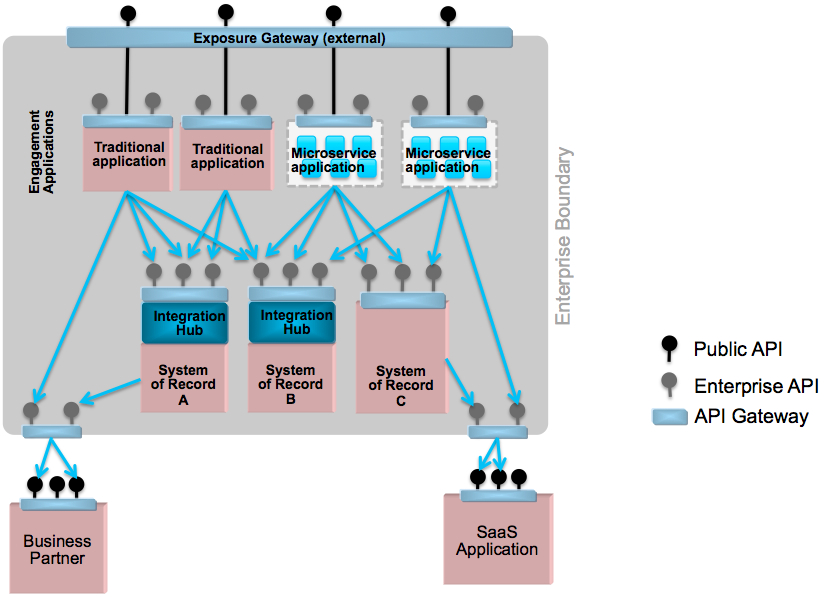
\includegraphics[width=\textwidth]{content/images/figure8}\
    \quelle\url{https://www.ibm.com/developerworks/websphere/library/techarticles/1601_clark-trs/1601_clark.html}
    \caption{Microservice, SOA und APIs Kombiniert}
    \label{fig:MicroservicesSOAAndAPIsCombined} 
\end{figure}

Möchte man eine Service-orientierte Architektur einsetzten, muss zunächst einmal die Frage gestellt werden, welcher Zweck damit erfüllt werden soll und welches Einsatzgebiet abgedeckt werden soll. Während mit Microservices die Entwicklung vereinfacht werden soll, wird mit SOA versucht die vorhandenen Unternehmensanwendungen zu strukturieren.
\\\\
Außerdem darf der Aufwand bei der Einführung eines neuen Architekturmusters nicht unterschätzt werden. Möchte ein Unternehmen beispielsweise SOA einführen, müssen alle Systeme im Unternehmen so angepasst werden, dass sie als Dienste verwendet werden können. Die Einführung von SOA betrifft somit das gesamte Unternehmen. Dabei ist das \textit{Gesetzt von Conway} zu beachten, wodurch häufig die Abteilungen eines Unternehmens neu strukturiert werden müssen, um SOA einzuführen. 

Bei der Einführung von einem Microservice-System betrifft diese Entscheidung zunächst einmal, nur ein Projekt, welches jedoch der Anfang von weiteren Microservice-Systemen sein kann.
\\\\
Zudem sollte nicht nur die Fragen nach dem Zweck gestellt werden, sondern auch nach den Einsatzmöglichkeiten. Wird ein System benötigt, welches einfach zu skalieren ist oder ein System, bei dem die Anwendungen besser strukturiert sind. Während in einem Microservice-System deutlich einfacher Skaliert werden kann, als in einem SOA-System, werden durch die Schnittstellen sehr viele Informationen bereitgestellt. Bei einem SOA-System hingegen wird dafür gesorgt, dass die Informationen gefiltert und aufbereitet werden, sodass der Nutzer nur die Informationen bekommt. Durch den Aufbau beider Muster, ist es jedoch möglich, durch hinzufügen oder ändern von Services, neue Geschäftsprozesse schneller zu etablieren.
\\\\
Ein wichtiger Punkt der Entscheidung ist die Wartbarkeit, solcher Systeme. Die Wartung muss ein aktiver Prozess in allen Stadien sein. Dies betrifft die Entwicklung, das Testen, das Deployment und die Skalierung. Zudem ist die Bindung an Technologie-Stacks ein wichtiges Thema. Möchte ein Unternehmen immer die neuste Technologie einsetzten, dürfte dies mit einem SOA-System schwieriger sein, als mit meinem Microservice-System.
\\\\
Abschließend kann man sagen, dass beide Paradigmen, zwar unterschiedliche Ansätze besitzen, jedoch das gleiche Ziel verfolgen: Das schnellere und einfachere Umsetzen von neuen Anforderungen. Dabei können beide Ansätze, aufgrund der unterschiedlichen Einsatzgebiete, gleichzeitig in einem Unternehmen eingesetzt werden. Bei der Einführung einer Service-orientierten Architektur, sollte gründlich analysiert werden, welche Eigenschaften das einzusetzende Paradigma erfüllen muss und wie viel Aufwand die Umsetzung bedeutet.

\section{Ausblick}
\label{sec:Ausblick}
In der Bachelorarbeit soll eine Anwendung, für die Zusammenarbeit, beispielhaft mit dem Microservice Paradigma erstellt werden. Anhand diesem beispielhaften System soll untersucht werden, welche Voraussetzungen gegeben sein müssen, um ein Microservice-System zu betreiben und welche Werkzeuge eingesetzt werden müssen, um ein Microservice-System aufzubauen, bzw. zu verwenden und zu verwalten. Konkret soll Untersucht werden, wie genau ein Microservice deployed und skaliert werden kann. Zudem soll untersucht werden wie Microservices in solch einem System gefunden und verwendet werden können. außerdem soll untersucht werden, wie die Benutzerverwaltung und die Authentifizierung in solch einem System funktioniert. Konkret soll untersucht werden, wie Benutzerberechtigungen verwaltet und abgefragt werden können, welche unterschiedlichen Ansätze dafür existieren und welche Vor- und Nachteile die jeweiligen Ansätze besitzen. Zusätzlich soll untersucht werden, wie das Monitoring in solch einem System funktioniert.

% ***************************** BIBLIOGRAPHY **********************************
\baselineskip=14pt
\addcontentsline{toc}{chapter}{\protect\numberline{}\bibname}
\bibliography{bib/thesis}

% ******************************* APPENDIX ************************************
%\appendix
%\baselineskip=18pt
%\chapter{Diagramme und Tabelle}
\label{chap:anhang_a}


% ***************************** BACK MATTER ***********************************
\pagestyle{empty}

\addcontentsline{toc}{chapter}{\protect\numberline{}Eidesstattliche Erklärung}
\chapter*{}
\vspace*{0.5cm}
\noindent
{\bf Eidesstattliche Erklärung} \\
Ich versichere an Eides statt, dass ich die vorliegende Arbeit selbständig
angefertigt und mich keiner fremden Hilfe bedient, sowie keine anderen als die
angegebenen Quellen und Hilfsmittel benutzt habe. Alle Stellen, die wörtlich
oder sinngemäß veröffentlichten oder nicht veröffentlichten Schriften und
anderen Quellen entnommen sind, habe ich als solche kenntlich gemacht. Diese
Arbeit hat in gleicher oder ähnlicher Form noch keiner Prüfungsbehörde
vorgelegen. 

\vspace{1cm}
\toponym, den \today \hfill \author


\vspace*{3cm}
\noindent
{\bf Erklärung} \\
Mir ist bekannt, dass nach § 156 StGB bzw. § 163 StGB eine falsche
Versicherung an Eides Statt bzw. eine fahrlässige falsche Versicherung an
Eides Statt mit Freiheitsstrafe bis zu drei Jahren bzw. bis zu einem Jahr oder
mit Geldstrafe bestraft werden kann. 

\vspace{1cm}
\toponym, den \today \hfill \author


%%%%%%%%%%%%%%%%%%%%%% NICHT IN ARBEIT ÜBERNEHMEN!!! %%%%%%%%%%%%%%%%%%%%%%%%%%
%\newpage
%\noindent
%\vspace*{6cm}
%\begin{center}
%{\bf Spezielle Erklärung vor Beginn der Bachelor-Thesis/Master-Thesis}
%\end{center}
%Hiermit erkläre ich, dass ich die vorausgehenden Seiten, die man sich unter 
%\\[0.2cm]
%{\scriptsize \bf \hspace*{0.3cm}ftp://gatekeeper.informatik.fh-dortmund.de/pub/professors/lenze/thesis/thesis.pdf} \\[0.2cm]
%ansehen kann, mit den Erläuterungen zum Aufbau, zum Umfang und zum Inhalt einer
%Bachelor-/Master-Arbeit sorgfältig 
%gelesen und verstanden habe. Insbesondere ist mir klar, was man unter
%wissenschaftlichem Arbeiten versteht und dass korrektes Zitieren ein
%wesentliches Element in diesem Zusammenhang ist. Alle Fragen, die es in diesem
%Kontext noch gab, habe ich inzwischen mit Herrn Lenze geklärt, und es bestehen
%keine Unklarheiten mehr. Über die besondere Problematik von Plagiaten und den
%Kriterien, die ein Vorliegen anzeigen, bin ich ebenfalls genau unterrichtet.
%
%\vspace{1.5cm}
%\toponym, den \\
%\ \ \  \ \ \hspace*{8cm} {\tiny Unterschrift!} \\
%
%\vfill

\end{document}
